\documentclass{article}

% if you need to pass options to natbib, use, e.g.:
%     \PassOptionsToPackage{numbers, compress}{natbib}
% before loading neurips_2020

% ready for submission
% \usepackage{neurips_2020}

% to compile a preprint version, e.g., for submission to arXiv, add add the
% [preprint] option:
%     \usepackage[preprint]{neurips_2020}

% to compile a camera-ready version, add the [final] option, e.g.:
%     \usepackage[final]{neurips_2020}

% to avoid loading the natbib package, add option nonatbib:
\usepackage[preprint]{neurips_2020}
\usepackage[utf8]{inputenc} % allow utf-8 input
\usepackage[T1]{fontenc}    % use 8-bit T1 fonts
\usepackage{hyperref}       % hyperlinks
\usepackage{url}            % simple URL typesetting
\usepackage{booktabs}       % professional-quality tables
\usepackage{amsfonts}       % blackboard math symbols
\usepackage{nicefrac}       % compact symbols for 1/2, etc.
\usepackage{microtype}      % microtypography
\usepackage{bbm}
%!TEX root =  autocontgrlp.tex

\usepackage{multicol}
\usepackage{multirow}
\usepackage{dsfont}
\usepackage{tabularx}
%\setlength{\marginparwidth}{13mm}
\usepackage[textsize=tiny]{todonotes}
%\usepackage[disable]{todonotes}
\newcommand{\todoch}[2][]{\todo[color=blue!20!white,#1]{C: #2}}
%\usepackage{enumitem}
%\usepackage[fleqn]{amsmath}
\usepackage{amsmath}
\usepackage{mathtools}
\usepackage{graphicx}
\usepackage{times}
\usepackage{helvet}
\usepackage{courier}
\usepackage{paralist}
\usepackage{latexsym}
\usepackage{url}
\usepackage[all]{xy}
\usepackage{amsmath}
\usepackage{amssymb}
\usepackage{amsthm}
\usepackage{nccmath} % mfrac
\usepackage{comment}
%\usepackage{enumitem}
\usepackage{paralist}
\usepackage{xcolor}
%\usepackage[colorlinks=true,linkcolor=blue,citecolor=purple]{hyperref}
%\usepackage{hyperref}
\usepackage{graphicx}
\usepackage{pifont}
%\usepackage{algorithm}
%\usepackage{algorithmic}
%\usepackage{pseudocode}
%\usepackage{algpseudocode}
\usepackage{savesym}
\savesymbol{AND}
\usepackage{xspace}
\usepackage{tikz}
\usepackage{pgfplots}
\usepackage{pgf}
\usepackage{algorithm}
\usepackage{algorithmic}
\usepackage{xspace}
\usepackage{comment}
\usepackage{placeins}
%\usepackage[capitalize]{cleveref}
%\usepackage{caption}

%\usepackage{style/ssltr}
%\usepackage{style/macros}
\if0
\usetikzlibrary{intersections}
\usetikzlibrary{arrows,calc,fit,patterns,plotmarks,shapes.geometric,shapes.misc,shapes.symbols,   shapes.arrows,   shapes.callouts,   shapes.multipart,   shapes.gates.logic.US,   shapes.gates.logic.IEC,   er,   automata,   backgrounds,   chains,   topaths,   trees,   petri,   mindmap,   matrix,   calendar,   folding, fadings,   through,   positioning,   scopes,   decorations.fractals,   decorations.shapes,   decorations.text,   decorations.pathmorphing,   decorations.pathreplacing,   decorations.footprints,   decorations.markings, shadows,circuits}
\tikzstyle{decision}=[diamond,draw]
\tikzstyle{line}=[draw]
\tikzstyle{elli}=[draw,ellipse]
\tikzstyle{arrow} = [thick]
\fi
%\usepackage{subfig}

\newcommand{\rsa}{\rightsquigarrow}

\newcommand{\mb}{\mbox{ }}
\newcommand{\one}{\mathbf{1}}
\newcommand{\zero}{\mathbf{0}}
\newcommand{\nn}{\nonumber}

\newcommand{\inrdnet}{\in\R^{d_{net}}}
\newcommand{\inrdin}{\in\R^{d_{in}}}
\newcommand{\R}{\Re} %{\mathbb{R}}
\newcommand{\Rm}{\mathbf{R}_{\min}}
\newcommand{\ra}{\rightarrow}
\newcommand{\om}{\otimes}
\newcommand{\op}{\oplus}
\newcommand{\RA}{\Rightarrow}
\newcommand{\LA}{\Leftarrow}
%\newcommand{\E}{\mathbb{E}}
\newcommand{\E}[1]{\mathbb{E}\left[#1\right]}
\newcommand{\lmin}[1]{\lambda_{\min}\left(#1\right)}
\newcommand{\T}{\mathcal{T}}
\newcommand{\B}{\mathcal{B}}
\newcommand{\F}{\mathcal{F}}
\newcommand{\C}{\mathcal{C}}
\newcommand{\M}{\mathcal{M}}
\newcommand{\N}{\mathcal{N}}

\newcommand{\I}{\mathcal{I}}

\newcommand{\mm}{m_{-}}
\newcommand{\mdm}{m'_{-}}
\newcommand{\Tvm}{\Theta^{v,\mm}}
\newcommand{\Tvmd}{\Theta^{v,\mdm}}


%\newcommand{\Tb}{\mathbf{\Theta}}
%\newcommand{\Tv}{\mathbf{\Theta}^v}
%\newcommand{\Tw}{\mathbf{\Theta}^w}
\newcommand{\tv}{\theta^v}

\newcommand{\Tb}{{\Theta}}
\newcommand{\Tv}{{\Theta}^v}
%\newcommand{\Tw}{{\Theta}^w}
\newcommand{\Tg}{{\Theta'}}

\newcommand{\tg}{\theta'}
%\newcommand{\Tg}{\mathbf{\Theta}^g}
\newcommand{\Tt}{\Theta}

\newcommand{\G}{\mathcal{G}}

\DeclareMathOperator{\argmin}{argmin}
\DeclareMathOperator{\argmax}{argmax}
\newcommand{\norm}[1]{\|#1\|}
\newcommand{\inorm}[1]{\|#1\|_{\infty}}
\newcommand{\snorm}[1]{\left\|#1\right\|}
\newcommand{\sinorm}[1]{\left\|#1\right\|_{\infty}}


%\newcommand{\eqdef}{\stackrel{\text{\footnotesize def}}{=}}
%\newcommand{\eqdef}{\stackrel{\Delta}{=}}
\newcommand{\eqdef}{\doteq}
\newcommand{\defeq}{\doteq}

\newcommand{\eps}{\varepsilon}
\renewcommand{\epsilon}{\varepsilon}

\newcommand{\nt}{\nabla_{\Theta}}
\newcommand{\al}{\mathcal{AL}}
\newcommand{\aw}{\mathcal{AW}}
\newcommand{\ap}{\mathcal{AP}}

\newcommand{\keywords}[1]{{\bf Keywords: } #1\par}
%\newenvironment{proof}{{\bf Proof:} }{}
\newtheorem{theorem}{Theorem}[section]
\newtheorem{lemma}{Lemma}[section]
\newtheorem{claim}[theorem]{Claim}
\newtheorem{proposition}[theorem]{Proposition}
\newtheorem{corollary}[theorem]{Corollary}
\newtheorem{assumption}{Assumption}
\newtheorem{definition}{Definition}[section]
\newtheorem{remark}{Remark}[section]
\newtheorem{identity}{Identity}[section]
\newtheorem{example}{Example}[section]
\newtheorem{note}{Note}[section]
\newtheorem{notation}{Notation}[section]
\newcommand{\alert}[1]{\textcolor{red}{#1}} 
\newcommand{\J}{\mathcal{J}}
\newcommand{\ip}[1]{\langle #1\rangle}

\def\v{\mathbf{v}}
\def\r{\mathbf{r}}
\def\p{\mathbf{p}}
\def\q{\mathbf{q}}
%\def\R{\mathrm{R}}
\def\Re{\mathbb{R}}
\def\Z{\mathbb{Z}}
\def\P{\mathcal{P}}
\def\S{\mathcal{S}}
\def\A{\mathcal{A}}
\def\X{\mathcal{X}}
\def\U{\mathcal{U}}

%\newcommand{\B}{\mathcal{B}}


\newcommand{\ith}[2][th]{$#2^{\text{#1}}$}
\newcommand{\us}[2]{\underset{#2}{#1}~}
\newcounter{subequation}[equation]
\newcommand{\thesubequationonly}{\alph{subequation}}
\renewcommand{\thesubequation}{\text{\theequation(\thesubequationonly)}}
\newcommand{\subequationitem}{\refstepcounter{subequation}(\thesubequationonly)\thinspace}

\def\mathdisplay#1{%
  \ifmmode \@badmath
  \else
    $\def\@currenvir{#1}%
    \let\dspbrk@context\z@
    \let\tag\tag@in@display \SK@equationtrue %\let\label\label@in@display
    \global\let\df@label\@empty \global\let\df@tag\@empty
    \global\tag@false
    \let\mathdisplay@push\mathdisplay@@push
    \let\mathdisplay@pop\mathdisplay@@pop
    \if@fleqn
      \edef\restore@hfuzz{\hfuzz\the\hfuzz\relax}%
      \hfuzz\maxdimen
      \setbox\z@\hbox to\displaywidth\bgroup
        \let\split@warning\relax \restore@hfuzz
        \everymath\@emptytoks \m@th $\displaystyle
    \fi
%   \fi
}

\newcommand{\algorithmicinput}{\textbf{Input:} }
\newcommand{\INPUT}{\item[\algorithmicinput]}
\newcommand{\algorithmicoutput}{\textbf{Output:} }
\newcommand{\OUTPUT}{\item[\algorithmicoutput]}
\newcounter{algostep}
\newcommand{\Step}[1][\STATE]{#1\textbf{\refstepcounter{algostep}\thealgostep}. }

\newenvironment{algoequation}{\refstepcounter{equation}$}{$\hfill (\theequation)}

\newenvironment{nonfloatalgorithm}[1]{\vspace{1ex}\hrule\vspace{0.5ex} \refstepcounter{algorithm}\textbf{Algorithm \thealgorithm}\hspace{1em} #1 \vspace{0.5ex}\hrule}{\hrule\vspace{1.5ex}\setcounter{algostep}{0}}

\newcounter{acalgorithm}

\newenvironment{nonfloatactorcriticalgorithm}[1]{\vspace{1ex}\hrule\vspace{0.5ex} \textbf{Actor-Critic Algorithm \refstepcounter{acalgorithm}\theacalgorithm}\hspace{1em} #1 \vspace{0.5ex}\hrule\addcontentsline{loa}{algorithm}{\protect\numberline{\theacalgorithm}{\ignorespaces #1}}}{\hrule\vspace{1.5ex}\setcounter{algostep}{0}}

\usepackage{hyperref}
\usepackage{thmtools}
\usepackage{nameref}

\usepackage[nameinlink,noabbrev,capitalize]{cleveref}
\crefname{assumption}{assumption}{assumptions}
\crefname{lemma}{lemma}{lemmas}
\Crefname{lemma}{Lemma}{Lemmas}
\crefname{thm}{theorem}{theorems}
\Crefname{thm}{Theorem}{Theorems}


\usepackage{caption}
\captionsetup{belowskip=0pt}
\usepackage{wrapfig,lipsum}
\usepackage[linewidth=1.2pt,linecolor=red]{mdframed}


\usepackage{comment}
\usepackage{cancel}
\usepackage{changepage}
\usepackage{bbm}
\usepackage{pgfplots}
\usepackage{filecontents}
\setcounter{MaxMatrixCols}{32}
\usepackage{placeins}

\title{Neural Path Features: Optimisation, Generalisation and Feature Learning}
% The \author macro works with any number of authors. There are two commands
% used to separate the names and addresses of multiple authors: \And and \AND.
%
% Using \And between authors leaves it to LaTeX to determine where to break the
% lines. Using \AND forces a line break at that point. So, if LaTeX puts 3 of 4
% authors names on the first line, and the last on the second line, try using
% \AND instead of \And before the third author name.
\author{Chandrashekar Lakshminarayanan and Amit Vikram Singh, \\ Indian Institute of Technology, Palakkad}
\begin{document}
\maketitle
\begin{abstract}
Understanding optimisation and generalisation in deep neural networks (DNNs) (with ReLU) trained using first-order method such as gradient descent (GD) is an important problem in machine learning. Recent works on this problem have made use of the \emph{neural tangent feature} (NTF) which is equal to the gradient of the DNN output with respect to its weights, i.e., the feature is based on first-order information. In this paper, we deconstruct the computation in DNNs into paths and gates. This deconstruction yields a novel zeroth-order feature namely the \emph{neural path feature} (NPF), whose dimension is equal to total the number of paths, and whose co-ordinate corresponding to a path is the product of the signal at its input node and its \emph{on/off} state\footnote{A path is \emph{on} if all the gates in the path are \emph{on}.}. We show that when optimising with fixed NPFs using GD i) increasing depth till a point helps in training and ii) increasing depth beyond a point hurts training. While in NTFs based works, DNNs are considered as linear learners with fixed NTF, we show via theory and experiments, that, in DNNs, NPFs are learnt during training, and such learning is key for generalisation. By bringing in zeroth-order information into the picture via NPFs, our work is complementary to prior work based on NTFs.
\end{abstract}
\begin{comment}
We study optimisation and generalisation in deep gated networks (DGNs), wherein, the output of a single hidden neuron is obtained as a product of its pre-activation input and a gating value. DNNs with ReLU activations are special cases of DGNs.  The DGN framework enables us to dismantle deep networks into paths and gates. This dismantling yields a novel (zeroth-order) \emph{neural path feature} (NPF) whose dimension is equal to total the number of paths, and whose co-ordinate corresponding to a path is the product of the signal at its input node and its \emph{on/off} state\footnote{A path is \emph{on} if all the gates in the path are \emph{on}.}. We show that the associated \emph{neural path kernel} (NPK) plays an important role in optimisation and generalisation of DGNs. %In particular, $H_t(x,x')=(x^\top x')\lambda_t(x,x')$, where $\lambda_t(x,x')$ is a count of total number of paths that are active simultaneously for both inputs $x,x'\in \R^{d_{in}}$. \hfill\\
For randomly initialised DGNs optimising with fixed NPFs, we show that i) increasing depth till a point helps in training and ii) increasing depth beyond hurts training. We verify via experiments that the NPFs are learned during training by showing that the norm of the labelling function measured with respect to the inverse of the trace normalised NPK reduces with time.
\end{comment}
\section{Introduction}
Understanding optimisation and generalisation in deep neural networks (DNNs) trained using first-order method such as gradient descent (GD) is an important problem in machine learning. Some of the recent works on this problem have made use of the \emph{neural tangent features} (NTFs) and the \emph{trajectory} based analysis. The NTF of an input $x\in \R^{d_{in}}$ is defined as $\psi_{x,t}=(\frac{\partial \hat{y}_{\Theta}(x)}{\partial \theta}|_{\Theta=\Theta_t},\theta \in \Theta)\in \R^{d_{net}}$, i.e., as the gradient of the network output $\hat{y}_{\Theta}(x)$ with respect to its weights $\Theta\inrdnet$. Since the NTF is a first-order term, it can be used to linearise the DNN output about the point $\Theta_t$. Associated with the NTF is a \emph{neural tangent kernel} (NTK), which is given by $K_t(x,x')=\psi^\top_{x,t}\psi_{x',t}$, where $x,x'\in\R^{d_{in}}$ are inputs to the DNN. In the \emph{trajectory} based analysis, one looks at the dynamics of error $e_t$  (i.e., difference between predicted and true values) at time $t$. For a small step-size $\alpha_t>0$ of the GD procedure, the error dynamics follows a recursion given by: $e_{t+1}=e_t-\alpha_tK_te_t$, where $K_t$ is the NTK matrix obtained on the the dataset. While it is known from \cite{dudnn}, that, gradient descent achieves zero training loss in over-parameterised DNNs, and from \cite{cao2019generalization}, that, the NTK at initialisation can be used to bound the generalisation performance, the following questions still remain unresolved: \hfill\\
\textbf{Question I (Optimisation):} \emph{What is the role of width and depth in training of DNNs? Why increasing depth till a point helps in training? Why increasing the depth beyond hurts training?}\\
The results by \cite{dudnn} only throw light on why ResNets could be better than fully connected DNNs. The above question in relation to fully connected networks is still unresolved.\\
\textbf{Question II (Generalisation):} \emph{What are the hidden features in a DNN? Are these features learned? and if so, how?} \hfill\\
There are couple of unresolved issues in prior work by \cite{arora2019exact,cao2019generalization}. Firstly, if the DNNs are only linear learners with random NTFs, then it means that, no feature learning happens in DNNs. Secondly, it was observed in prior experiments, that, the DNNs perform better than their corresponding NTK counterparts \cite{arora2019exact,lee2017deep}. \hfill\\
\textbf{Our Contributions:} In this paper, we study fully connected deep gated networks (DGNs), with $d$ layers, and $w$ hidden units per layer. In a DGN,  the output of a single hidden unit is given by the product of its pre-activation input and its gating value. DNNs with ReLU activations are special cases of DGNs. Central idea in this paper is the `path-view': to regard paths and gates as basic building blocks of a DGN. A \emph{path} starts from an input node, passes through exactly one weight and one activation in each layer, and finally ends at the output node. Let $[P]=\{1,\ldots,P\}$ be an enumeration of all the paths, the zeroth and first order quantities of a DNN can then be expressed as:
\begin{align}
\label{eq:zero}&\text{(Zeroth-Order/Neural Path Feature)}&\quad:& \quad \hat{y}_t(x)={\phi^\top_{x,t}} v_t=\sum_{p\in [P]}x(\I(p))A_t(x,p)v_t(p)\\
%\text{(First Order)}\quad: \quad \partial \hat{y}_t(x)&= \sum_{p\in [P]}x(\I(p)) A_t(x,p) \partial((v_t(p))+\sum_{p\in [P]}x(\I(p)) \partial(A_t(x,p)) v_t(p)\nn\\
\label{eq:first}&\text{(First- Order/Neural Tangent Feature)}&\quad:&\quad   \nabla \hat{y}_t(x)=\psi_{x,t}=(\nabla v_t )^\top \phi_{x,t} + (\nabla \phi_{x,t})^\top v_t,
\end{align}
where, for a path $p$, $\I(p)$ is the input node at which it starts, $v_t(p)$ is its value given by the product of its weights and for input $x\in\R^{d_{in}}$, $A_t(x,p)$ is its activation level given by the product of the gating values in the path. In order to understand the role $A_t$, we handle the gating values as independent variables\footnote{In a DNN with ReLU activations, the gates are implicit: a gate is \emph{on} only if pre-activation input is positive.}. We now list the major highlights in the paper.\hfill\\
$1.$ \textbf{Information Flow:} We introduce a host of novel terms/expressions and concepts related to information flow in DGNs. This includes i) the zeroth-order (see \eqref{eq:zero}) \emph{neural path feature} (NPF) and the \emph{neural path kernel} (NPK) denoted by $H_t$, which are defined using the gating information, ii) the first-order (see \eqref{eq:first}) terms namely, the \emph{value gradient} given by $(\nabla v_t )^\top \phi_{x,t}$, and the \emph{feature gradient} given by $(\nabla \phi_{x,t})^\top v_t$, iii)  two sub-network of paths namely, an \emph{active} sub-network, which is the set of active paths that hold the memory for an input, through which the value gradient flows and a \emph{sensitive} sub-network, which is the set of sensitive paths, through which the feature gradient flows. We also show that for random initialisation, the paths exhibit a \emph{disentanglement} property, which is very key in our results.\\
%$1.$ \textbf{Representation and Generalisation:} By fixing the activation (i.e., $A_t=A_0,\forall t\geq 0$), we train DGNs with different fixed \emph{neural path features} (NPFs), and demonstrate that the NPFs are key for generalisation. Further, we show that the NPFs are learnt during training. This shows that NPFs can be regarded as the true hidden features in a deep network.\\
$2.$ \textbf{NPFs and Optimisation:}  When the weights are randomly initialised (with an appropriate scale) in a manner statistically independent of the gates, we show that, $\E{K_0}=H_0$, and $Var\left[K_0(x,x')\right]\leq O(\max\{\frac{d^2}{w}, \frac{d^3}{w^2}\})$. We argue that  $H_0$ whitens with depth, and hence, increasing depth helps in training. Increasing depth further causes $K_0$ to deviate from $H_0$, and hence, degrades the spectrum of $K_0$, thereby affecting training performance.\\
$3.$ \textbf{NPFs and Generalisation:} By fixing the activation (i.e., $A_t=A_0,\forall t\geq 0$), we train DGNs with different fixed NPFs, and demonstrate that the NPFs are key for generalisation. Further, we show that the NPFs are learnt during training. This shows that NPFs can be regarded as the true hidden features in a deep network.\\
$4.$ \textbf{NPF Learning:} We present preliminary results connecting NPF learning and the trajectory method.

\begin{comment}
Understanding optimisation and generalisation of deep neural networks (DNNs) trained using first-order method such as (stochastic) gradient descent is an important problem in machine learning. In this paper, we throw light on the following two questions:\hfill\\
\textbf{Question I (Optimisation):} \emph{What is the role of width and depth in training of DNNs? Why increasing depth till a point helps in training? Why increasing the depth beyond hurts training?}\\
\textbf{Question II (Generalisation):} \emph{What are the hidden features in a DNN? Are these features learned? and if so, how?} \hfill\\

\textbf {Background:} We consider a fully connected deep gated network (DGN) of depth $d$, and width $w$, weights $\Theta\in\R^{d_{net}}$, which, accepts an input $x\in \R^{d_{in}}$ and produces an output $\hat{y}_{\Theta_t}(x)\in \R$. In a DGN, the output of a hidden neuron is obtained as a product of its pre-activation input and a gating value. DNNs with ReLU activations are special cases DGNs. Some of the recent works to understand SGD in relation to the optimisation and generalisation in DNNs make use of the \emph{neural tangent features} (NTFs) and the \emph{trajectory} based analysis, which we describe in brief.\hfill\\
$1.$The NTF for an input $x\in \R^{d_{in}}$ is defined as $\psi_{x,t}=(\frac{\partial \hat{y}_{\Theta}}{\partial \theta}|_{\Theta=\Theta_t},\theta \in \Theta)\in \R^{d_{net}}$, i.e., collection of the gradients of the network output with respect to its weights. Since the NTF is a first-order term, it can be used to linearise the DNN output about the point $\Theta_t$. Associated with the NTF is a \emph{neural tangent kernel} (NTK), which is given by $K_t(x,x')=\psi^\top_{x,t}\psi_{x',t}$. 
$2.$ In the \emph{trajectory} based analysis, one looks at the dynamics of error $e_t$  (i.e., difference between predicted and true values) at time $t$. For a small step-size $\alpha_t>0$, the error dynamics follows a linear recursion given by: $e_{t+1}=e_t-\alpha_tK_te_t$, where $K_t$ is the NTK matrix obtained on the the dataset. Thus, the spectral properties of $K_t$ is key to achieve zero training error. \hfill\\
\textbf{Related Work and Gaps:} \hfill\\
\emph{Optimisation:} \cite{ntk} were the first to point out the role of NTK in DNNs. Using the trajectory based analysis, \cite{dudnn} show that in fully connected DNNs with $w=\Omega(poly(n)2^{O(d)})$, and in residual neural networks (ResNets) with $w=\Omega(poly(n,d))$ gradient descent converges to zero training loss.  However, Question I, i.e., `why depth helps in training?' is unresolved.\hfill\\%This shows that ResNets are better than fully connected DNNs, based on the fact that the dependence on the number of layers improves exponentially for ResNets. 
\emph{Generalisation:} \cite{arora2019exact,arora,cao2019generalization} use NTK to provide generalisation bounds as well as propose pure-kernel methods. However, couple of issues remain unresolved: firstly, if the DNNs are only linear learners with random NTFs, then it suggests that no feature learning happens in DNNs, and secondly, it was observed in prior experiments that the DNNs perform better than their corresponding NTK counterparts \cite{arora2019exact,lee2017deep}. \hfill\\

\textbf{Our Results:} We now highlight the contributions in this paper.\\
$1.$ \textbf{Neural Path Feature:} Central idea in this paper is the `path-view': to regard paths and gates as basic building blocks of a DGN.  A \emph{path} starts from an input node, passes through exactly one weight and one activation in each layer, and finally ends at the output node. Let $[P]=\{1,\ldots,P\}$ be an enumeration of all the paths, then the \emph{neural path feature} (NPF) is defined $\phi_{x,t}=(x(\I(p))A_t(x,p),p\in[P])\in\R^P$, wherein, for a path $p$, $\I(p)$ is the input node at which it starts, and  $A_t(x,p)$ is its activation level is equal to the product of the gating values in the path. Using the NPF, the output is expressed as $\hat{y}_t(x)=\phi^\top_{x,t}v_t$, where, $v_t=(v_t(p),p\in[P])\in \R^P$, with $v_t(p)$ is the value of a path $p$ and is equal to the product of its weights.\hfill\\
$2.$ \textbf{Neural Path Kernel (NPK)}  is given by $H_t(x,x')=\phi^\top_{x,t}\phi_{x',t}$, where $x,x'\in\R^{d_in}$ are the inputs to the DGN. We show that the NPK whitens as depth increases.\hfill\\
$3.$ \textbf{Optimisation:}  When weights are initialised at random (with variance $\sigma$) and statistically independent of the activations, we show that $\E{K_0}= CH_0$, (for some constant $C>0$) and  $Var\left[K_0(x,x')\right]\leq O(\max\{\frac{d^2}{w}, \frac{d^3}{w^2}\})$ (for $\sigma^2=O(\frac{1}w)$). Thus,\\
(i) For a fixed $d$, increasing $w$ ensures $K_0$ converges to $\E{K_0}$, and since NPK matrix whitens as depth increases, increasing depth till a point helps in training performance.\hfill\\
(ii) For a fixed $w$, increasing $d$ makes the entries of $K_0$ deviate from $\E{K_0}$, thus degrading the spectrum of $K_0$. Thus increasing depth beyond a point hurts training performance. \hfill\\
$4.$ \textbf{Feature Learning:} Since $\hat{y}_t(x)=\phi^\top_{x,t}v_t$, the gradient flow has two components: an $(\nabla v_t)^\top\phi_{x,t}$ term, which we call the \emph{value gradient}, learns the path values (which are akin to weight vector in a standard linear approximation) keeping the NPFs fixed, and a $(\nabla \phi_{x,t})^\top v_t $ term, which we call the \emph{feature gradient} learns the NPFs keeping the path values fixed. We present preliminary theory connecting the trajectory method and feature learning. \hfill\\
$5.$ \textbf{Generalisation:} We experiment with two gating regimes namely the static, wherein, $A_t=A_0,\forall t \geq 0$, and the dynamic, wherein $A_t$ changes during training. The experiments on MNIST and CIFAR show that, better generalisation happens when the activations $A_t$ change with time. In particular, for binary classification, we verify that the quantity $y^\top (\widehat{H_t})^{-1}y$\footnote{For a matrix $H$, $\hat{H}=\frac{1}{trace(H)}H$ .} reduces as the training progresses. This shows that the eigenspaces of the NPK matrix align themselves in accordance to the labelling function. These experiments supports the fact that NPF and the NPK are indeed learnt during training in a manner to improve the generalisation performance. \hfill\\
\end{comment}
\begin{comment}
\textbf{Paths:}  A \emph{path} starts from an input node, passes through exactly one weight and one activation in each layer, and finally ends at the output node. Let $[P]=\{1,\ldots,P\}$ be an enumeration of all the paths, the zeroth and first order quantities of a DNN can then be expressed as:
\begin{align}
\label{eq:zero}\text{(Zeroth Order)}\quad: \quad \hat{y}_t(x)&=\sum_{p\in [P]}x(\I(p))A_t(x,p)v_t(p)={\phi^\top_{x,t}} v_t\\
\text{(First Order)}\quad: \quad \partial \hat{y}_t(x)&= \sum_{p\in [P]}x(\I(p)) A_t(x,p) \partial((v_t(p))+\sum_{p\in [P]}x(\I(p)) \partial(A_t(x,p)) v_t(p)\nn\\
\label{eq:first}\psi_{x,t}=(\partial v_t)^\top\phi_{x,t}+ (\partial \phi_{x,t})^\top v_t,
\end{align}
where, for a path $p$, $\I(p)$ is the input node at which it starts, $v_t(p)$ is its value given by the product of its weights and for input $x\in\R^{d_{in}}$, $A_t(x,p)$ is its activation level given by the product of the gating values in the path. \hfill\\
\textbf{Independent Gates and Activations:} In order to understand the role $A_t$, we handle the gating values as independent variables\footnote{In DNN with ReLU, the gates are implicit: a gate is \emph{on} only if pre-activation input is positive.}. All the theoretical results are under the assumption that $A_0$ is statistically independent of $\Theta_0$. \hfill\\
\textbf{Neural Path Feature and Kernel:} The \emph{neural path feature} (NPF) is given by $\phi_{x,t}=(x(\I(p))A_t(x,p))\in \R^P$ (see \eqref{eq:zero}) , and an associated \emph{neural path kernel} (NPK) to $H_t(x,x')=\phi^\top_{x,t}\phi_{x',t}$. The NPK has special structure: $H_t(x,x')=(x^\top x')\lambda_t(x,x')$, where $\lambda_t(x,x')$ is a measure of similarity based on the path activation levels for inputs $x,x'\in\R^{d_{in}}$. \hfill\\
\textbf{NPK vs NTK: } Under symmetric Bernoulli initialisation, we have $\E{K_0} = C H_0$, ($C>0$ is a constant), where $K_0$ is the NTK matrix at $t=0$. \hfill\\
\textbf{Optimisation I:} We argue that $\frac{\lambda_0(x,x')}{\lambda_0(x,x)}$ decays at an exponential rate with depth, i.e., the Gram matrix $K_0$ whitens with depth. Thus increasing depth helps in training. \hfill\\
\textbf{Optimisation II:} We show that $Var\left[K_0(x,x')\right]\leq O(\max\{\frac{d^2}{w}, \frac{d^3}{w^2}\})$ (for $\sigma^2=O(\frac{1}w)$). For a fixed $d$, increasing $w$ ensures $K_0$ converges to $\E{K_0}$. However, for a fixed $w$, increasing $d$ makes the entries of $K_0$ deviate from $\E{K_0}$, thus degrading the spectrum of $K_0$. Thus increasing depth beyond a point hurts training performance. \hfill\\
\textbf{Generalisation:} We experiment with two gating regimes namely the static, wherein, $A_t=A_0,\forall t \geq 0$, and the dynamic, wherein $A_t$ changes during training. The experiments on MNIST and CIFAR show that, better generalisation happens when the activations $A_t$ change with time. In particular, for binary classification, we verify that the quantity $y^\top (\widehat{H_t})^{-1}y$\footnote{For a matrix $H$, $\hat{H}=\frac{1}{trace(H)}H$ .} reduces as the training progresses. This shows that the eigenspaces of the NPK matrix align themselves in accordance to the labelling function. These experiments supports the fact that NPF and the NPK are indeed learnt during training in a manner to improve the generalisation performance. \hfill\\
\end{comment}
\section{Deep Gated Network}\label{sec:pathgate}
\FloatBarrier
\begin{table}[h]
\begin{minipage}{0.5\columnwidth}
\resizebox{\columnwidth}{!}{
\begin{tabular}{|l|l|}\hline
\multicolumn{2}{|c|}{Deep Gated Network: $\N(\Theta_t;\G_t)$}\\\hline 
Input layer & $z_{x,\Theta_t}(0)=x$ \\\hline
Pre-activation & $q_{x,\Theta_t}(l)={\Theta_t(l)}^\top z_{x,\Theta_t}(l-1)$\\\hline
Layer output & $z_{x,\Theta_t}(l)=q_{x,\Theta_t}(l)\odot G_{x,t}(l)$ \\\hline
Final output & $\hat{y}_t(x)={\Theta_t(d)}^\top z_{x,\Theta_t}(d-1)$\\\hline
Gating Values& $\begin{aligned}\G_t\stackrel{def}=\{G_{x_{s},t}(l,i), \forall s\in[n],\\l\in[d-1],i\in[w]\}\end{aligned}$\\\hline
\end{tabular}
}
\end{minipage}
\begin{minipage}{0.5\columnwidth}
\resizebox{\columnwidth}{!}{
\begin{tabular}{|c|c|}\hline
Gating Network: $\G(\Tg_t,\beta)$\\\hline
$z_{x,\Tg_t}(0)=x$  \\\hline
$q_{x,\Tg_t}(l)={\Tg_t(l)}^\top z_{x,\Tg_t}(l-1)$ \\\hline
$z_{x,\Tg_t}(l)=q_{x,\Tg_t}(l)\odot G_{x,\Tg_t}(l)$ \\\hline
{$\begin{aligned}\beta >0: G_{x,\Tg_t}(l,i)&=\frac{1+\epsilon}{1+\exp(-\beta q_{x,\Tg_t}(l,i))} \\ \beta=\infty: G_{x,\Tg_t}(l,i)&=\mathbbm{1}_{\{q_{x,\Tg_t}(l,i)>0\}}\end{aligned}$}\\\hline 
\end{tabular}
}
\end{minipage}
\caption{Here $\Theta(l,i,j)$ denotes the weight connecting node $i$ of layer $l-1$ to node $j$ of layer $l$, and $\odot$ stands for the \emph{Hadamard} product. The left table shows a DGN, and the right table shows a gating network. }
\label{tb:dgn}
\end{table}
We denote the dataset is given by $(x_s,y_s)_{s=1}^n$, the data matrix is given by $x=(x_s,s\in[n])\in\R^{d_{in}\times n}$, and $y_s\in\R$ in the case of regression and $y_s\in[C]$ in the case of $C$-class classification. Further, let $y=(y_s,s\in[n])$ be the vector of labels. We consider fully connected deep gated networks with $d$ layers (i.e., depth $=d$), and $w$ hidden units per layer (i.e., width $=w$). In \Cref{tb:dgn}, $q(l),z(l)$ and $G(l)$ are $w$-dimensional quantities, where $G(l)$ are the gating values.  At at time $t$, by specifying the gating values for all the $n$ input examples as $\G_t\stackrel{def}=\{G_{x_{s},t}(l,i), \forall s\in[n],l\in[d-1],i\in[w]\}$, we can recover the outputs $\hat{y}_t(x_s)\in \R$ for all the inputs $\{x_s\}_{s=1}^n$ in the dataset.  A DGN is denoted by $\N(\Theta_t;\G_t)$, i.e., the weights and the gating values are decoupled, and need to be specified to obtain a complete description. The gating values can also be obtained from a different gating network, parameterised by $\Tg\inrdnet$: we denote the gating values by $\G(\Tg_t,\beta)$. We also consider soft-gating, which uses a sigmoidal function: desirable feature here is that the gating values are differentiable with respect to the underlying parameter. Following the notational conventions, a DNN with ReLU activations is denoted by $\N(\Theta_t;\G(\Theta_t,\infty))$.\begin{comment}
The DGN framework allows us the flexibility to study a host of deep networks with different gating mechanisms. The gates can be fixed (i.e., $\G_t=\G_0,\forall t\geq 0$) or learnable, i.e., $\G_t$ changes during training. The gates can be parameterised explicitly with $\Tg\neq \Theta$, or implicitly with $\Tg=\Theta$, or unparameterised. Further, the gating can be hard taking values in $\{0,1\}$ or soft taking values in $(0,1+\epsilon)$.
\end{comment}
\begin{figure}
%\begin{minipage}{0.78\columnwidth}
\resizebox{\columnwidth}{!}{
\begin{tabular}{ccc}
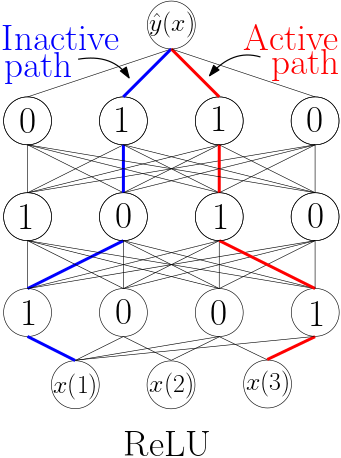
\includegraphics[scale=0.5]{figs/nn.png}
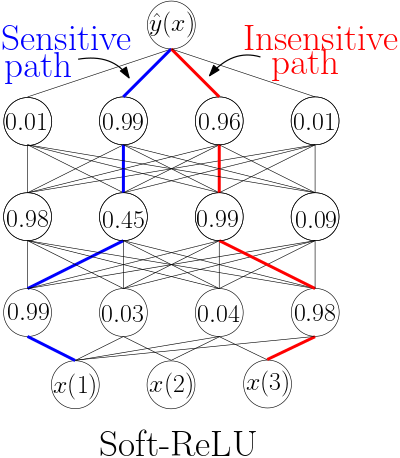
\includegraphics[scale=0.5]{figs/nnsoft.png}
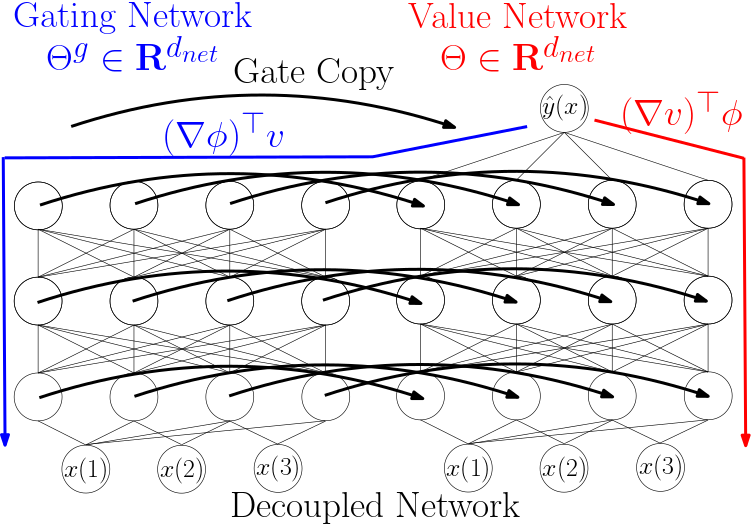
\includegraphics[scale=0.5]{figs/nntwin.png}
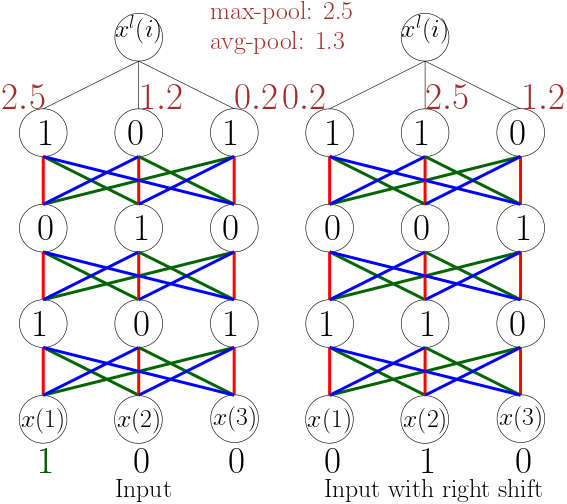
\includegraphics[scale=0.5]{figs/nnconv.png}
%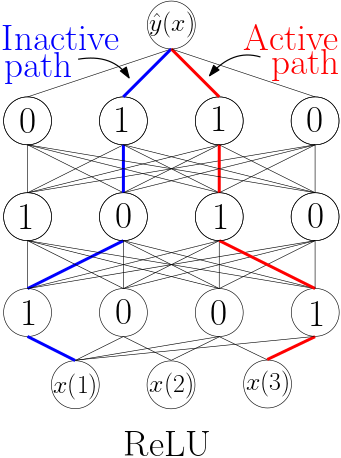
\includegraphics[scale=0.5]{figs/nn.png}
%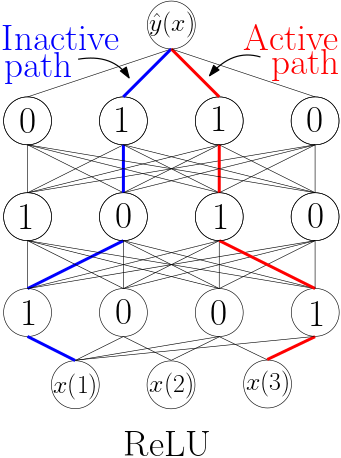
\includegraphics[scale=0.5]{figs/nn.png}
\end{tabular}
}
%\end{minipage}
%\begin{minipage}{0.18\columnwidth}
%\resizebox{\columnwidth}{!}{
%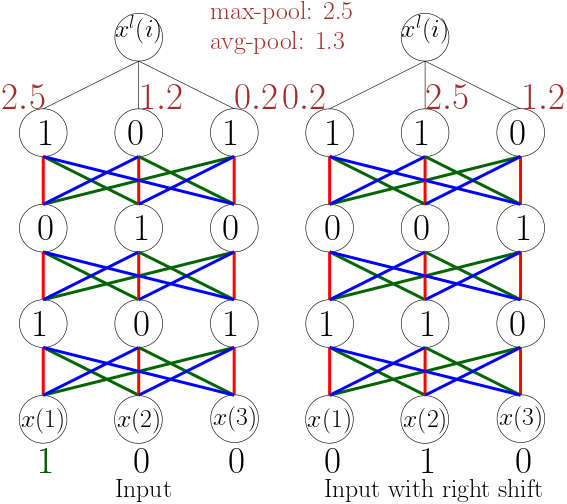
\includegraphics[scale=0.5]{figs/nnconv.png}
%}
%\end{minipage}

\end{figure}

%\section{Features and Kernels: Zeroth- vs First-Order}
\textbf{Zeroth-Order:} We first discuss zeroth-order neural path feature (NPF) and kernel (NPK), and then connect it to the first-order neural tangent feature  (NTF)and kernel (NTK).\hfill\\
The \emph{neural path feature} of an input $x\in \R^{d_{in}}$ is given by $\phi_{x,t}=(x(\I_0(p))A_t(x,p) ,p\in[P])\in\R^P$. By arranging the NPF of the $n$ input examples in a matrix $\Phi_t=\left[\phi_{x_1,t},\ldots, \Phi_{x_n,t}\right]$, we can express the predicted output of a DGN as: \begin{align}\label{eq:npfbasic}\hat{y}_t=\Phi_t^\top v_t,\end{align}
where, the value of the path $v_t$ is the equivalent of the so called \emph{weight-vector} in a standard linear approximation. The significance of the NPF are:\hfill\\
$1.$ \textbf{Signal-Wire Separation}: Note that $\Phi$ encodes the signal: say for a DNN with ReLU activations, the co-ordinate corresponding to path $p$ is either $x(p(0))$ if the path is active for that input (i.e., $A_t(x,p)=1$) or $0$ if the path is inactive for that input  (i.e., $A_t(x,p)=0$). The value of the path thus encodes the \emph{wire}, i.e., the information contained in the weights of the network. \hfill\\
$2.$ \textbf{Deep Information Propagation:} The path view provides a novel way of looking at information propagation in DNNs, eschewing the conventional `layer-by-layer' expression for information flow.\hfill\\
\begin{definition}\label{def:lambda}
 For any $i\in [d_{in}]$ define $\lambda_t(s,s')\stackrel{def}{=}\sum_{p\rsa i} A_t(x_s,p) A_t(x_{s'},p)$.
 \end{definition} 
$\lambda_t(s,s')$, is to be understood as the measure of activation similarity of the paths for inputs $s,s'\in[n]$. Here, $\lambda_t$ counts the total number of paths that are simultaneously \emph{on/active} for both inputs $s,s'\in[n]$. Note that the definition of $\lambda_t$ is independent of $i\in [d_{in}]$: owing to symmetry the same number of paths start from any given input node, and see exactly the same gates in the subsequent layers.
\begin{lemma}\label{lm:npk}[Neural Path Kernel] Let $x=(x_s,s\in [n])\in\R^{d_{in}\times n}$ be the data matrix and let the neural path kernel matrix be defined as $H_t\stackrel{def}=\Phi^\top_t\Phi_t$. It follows that $H_t= (x^\top x)\odot(\lambda_t)$. \end{lemma}
\textbf{First-Order:} The \emph{neural tangent feature} (NTF) $\psi_{x,t}\in \R^{d_{net}}$ is given by the gradient of the output with respect to the network parameters. From \eqref{eq:npfbasic} it follows that $\psi_{x,t}=(\partial \phi_{x,t})^\top v_t +(\partial v_t)^\top\phi_{x,t}$. In what follows (in the current section and next section), we assume that the gates are frozen, i.e., $\G_t=\G_0, A_t(\cdot,\cdot)=A_0(\cdot,\cdot),\forall t\geq 0$, and hence $\partial \phi_{x,t}=0$.\hfill\\
\textbf{Value Tangent Feature:} For a path $p$, the gradient  $\partial v_t(p)$ is given by: \begin{align}\label{eq:vft}{\partial v_t(p)}/{\partial \Theta\left(l,\I_{l'-1}(p),\I_{l'}(p)\right)}|_{\Theta=\Theta_t}= \underset{l=1}{\underset{l\neq l'}{\overset{d}{\Pi}}} \Theta_t\left(l,\I_{l-1}(p),\I_{l}(p)\right)\end{align} The gradient of the value of a path $p$ with respect to the $d_{net}$ parameters can be collected in a \emph{value tangent feature} (VTF) denoted by $\varphi_{p,t}\in \R^{d_{net}}$. Note that, from \eqref{eq:vft} it follows that the VTF entry corresponding to a weight is $0$ if the path $p$ does not pass through that weight, and hence $\varphi_{p,t}$ has a maximum of $d$ non-zero entries.\hfill\\

\begin{assumption}\label{assmp:main}
(i) $\G_0$ is statistically independent of $\Theta_0$, and (ii) $\Theta_0\stackrel{iid}\sim Ber\left(\frac{1}{2}\right)$ over the set $\{-\sigma,+\sigma\}$. 
\end{assumption}
\begin{lemma}\label{lm:disentangle}[Disentanglement]
Under \Cref{assmp:main}, for paths $p,p'\in \P, p\neq p'$, we have  i) $\E{\ip{\varphi_{p,0}, \varphi_{p',0}}}= 0$ and ii)${\ip{\varphi_{p,0}, \varphi_{p,0}}}= d\sigma^{2(d-1)}$.
\end{lemma}
\begin{theorem}\label{th:exp}[NTK and NPK]
$\E{K_0}=d\sigma^{2(d-1)}(x^\top x) \odot (\lambda_0)$.
\end{theorem}
\begin{proof} Let $\varphi_t=\left[\varphi_{p,t},p\in[P]\right]\in\R^{d_{net}\times P}$ be the VTF matrix at time $t$, then if follows that the NTK (Gram) matrix is  $K_t=\Psi^\top_t\Psi_t=\Phi^\top_t\varphi_t\varphi^\top_t\Phi_t$. Now, taking expectation we have $\E{K_0}=\E{\Phi^\top_t\varphi_t\varphi^\top_t\Phi_t}$, and using \Cref{assmp:main}-(i), one can pull out the $\Phi_t$ terms outside of the expectation, i,e., $\E{K_0}=\Phi^\top_t\E{\varphi_t\varphi^\top_t}\Phi_t$, and using \Cref{assmp:main}-(ii), we can show that $\E{\varphi_t\varphi^\top_t}=d\sigma^{2(d-1)}I$. The statement of \Cref{th:exp} follows by using \Cref{lm:npk}.
\end{proof}
\begin{theorem}\label{th:var}
Under \Cref{assmp:main} and the condition that ${4d}/{w^2}<1$, it follows that\hfill\\
$Var\left[K_0\right]\leq O\left(d^2_{in}\sigma^{4(d-1)}\max\{d^2w^{2(d-2)+1}, d^3w^{2(d-2)}\}\right)$.

\end{theorem}
%\section{Learning with Neural Path Features}
\begin{comment}
\textbf{NPFs and Optimisation:} The ability of DNNs to fit data has been demonstrated in the past \cite{ben}, i.e., they can fit even random labels, and random pixels of standard datasets such as MNIST. However, for standard DNNs with ReLU gates, with no bias parameters, a dataset with $n=2$ points namely $(x,1)$ and $(2x,-1)$ for some $x\in \R^{d_{in}}$ cannot be memorised. The reason is that the gating values are the same for both $x$ and $2x$ (for that matter any positive scaling of $x$), and hence $\phi_{2x,\G_t }= 2\phi_{x,\G_t }$, and thus it not possible to fit arbitrary values for $\hat{y}_t(x)$ and $\hat{y}_t(2x)$.\\
\end{comment}
 We trained DGN on standard datasets namely MNIST and CIFAR-10, under the following conditions: i) the gates are frozen $\G_t=\G_0,\forall t\geq 0$ and ii) the gating values are obtained from a ReLU network, which acts as the gating network (see \Cref{tb:dgn}). Since, the gates are frozen, the NPFs are fixed and the SGD learns only the path values. We compare the performance of $4$ different NPFs, wherein, the gates are copied from i) from a randomly initialised ReLU network (untrained), ii) from a ReLU network trained with good dataset iii) ReLU network trained on random labels and iv) ReLU network trained on random pixels.
\FloatBarrier
\begin{table}[h]
\begin{tabular}{|c|c|c|c|c|c|c|}\hline
&&&&\multicolumn{3}{c|}{NPF (trained)}\\\cline{5-7}
$(w,d)$	&Dataset		&ReLU		&NPF(untrained) 		&Good 		&Random Labels 	&Random Pixel\\\hline
$(128,6)$	& MNIST 		& $98.15$ 		&$96$ 		&$98.3$		&$92.6$			&$94.3$\\\hline
$(256,6)$	& MNIST 		& $98.5$ 		&$96.6$ 		&$98.4$		&$92.0$			&$81.1$\\\hline
\end{tabular}
\caption{Shows the training and generalisation performance of various GaLU network. Here, non-learned stands for gates from a randomly initialised ReLU network.}
\label{tb:npfs}
\end{table}
\FloatBarrier
\begin{wrapfigure}{h}{0.3\textwidth}
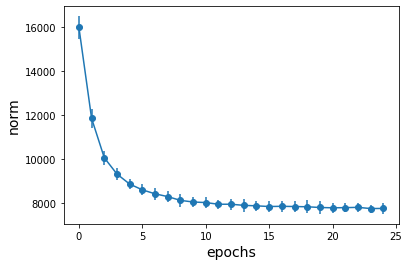
\includegraphics[scale=0.25]{figs/path-gram.png}
\caption{\label{fig:frog1}This is a figure caption.}
\end{wrapfigure}
\textbf{NPF dynamics:} We consider ``Binary''-MNIST data set with two classes namely digits $4$ and $7$, with the labels taking values in $\{-1,+1\}$ and squared loss. We trained a standard DNN with ReLU activation ($w=100$, $d=5$). Recall that $H_t=\Phi^\top_t\Phi_t$  (the Gram matrix of the features) and let $\widehat{H}_t=\frac{1}{trace(H_t)}H_t$ be its normalised counterpart. For a subset size, $n'=200$ ($100$ examples per class) we plot $\nu_t=y^\top (\widehat{H}_t)^{-1} y$, (where $y\in\{-1,1\}^{200}$ is the labeling function), and observe that $\nu_t$ reduces as training proceeds (see first plot in \Cref{fig:gen}). Note that $\nu_t=\sum_{i=1}^{n'}(u_{i,t}^\top y)^2 (\hat{\rho}_{i,t})^{-1}$, where $u_{i,t}\in \R^{n'}$ are the orthonormal eigenvectors of $\widehat{H}_t$ and $\hat{\rho}_{i,t},i\in[n']$ are the corresponding eigenvalues. Since $\sum_{i=1}^{n'}\hat{\rho}_{i,t}=1$, the only way $\nu_t$ reduces is when more and more energy gets concentrated on $\hat{\rho}_{i,t}$s for which $(u_{i,t}^\top y)^2$s are also high. However, in $H_t=(x^\top x)\odot \lambda_t$, only $\lambda_t$ changes with time. Thus, $\lambda_t(s,s')$ which is a measure of overlap of sub-networks active for input examples $s,s'\in[n]$, changes in a manner to reduce $\nu_t$. We can thus infer that the \emph{right} active sub-networks are learned over the course of training. We now summarise the insights obtained from these experiments in the following remarks:\hfill\\

\section{Main Result}
In this section, we assume that the NPKs are given to us and fixed (i.e, $G_t=\G_0,\forall t\geq 0$ is given to us). We show that, at randomised weight initialisation, the NTK is equal to (but for a scaling factor) to the NPK. We then use the \emph{Hadamard} structure of the NPK to comment about optimisation and generalisation. 
\begin{assumption}\label{assmp:main}
(i) $\Theta_0\inrdnet$  is statistically independent of $\G_0$ and (ii) The weights $\Theta_0$ are sampled i.i.d from a distribution such that for any $\theta_0\in\{\Theta_0\cup \Tg_0\}$,  we have $\E{\theta_0}=0$, and  $\E{\theta^2_0}=\sigma^2$, and $\E{\theta^4_0}={\sigma'}^2$.
\end{assumption}
\begin{theorem}\label{th:main} Under \Cref{assmp:main}, we have:\\
(i) $\E{K_0}=\sigma^{2(d-1)}H_0=\sigma^{2(d-1)}(x^\top x)\odot(\lambda_0)$,\\
(ii) In addition, if ${4d}/{w^2}<1$, then $Var\left[K^v_0\right]\leq O\left(d^2_{in}\sigma^{4(d-1)}\max\{d^2w^{2(d-2)+1}, d^3w^{2(d-2)}\}\right)$,\\
\end{theorem}
\begin{comment}
\textbf{Proof of \Cref{th:main}-(i):} Let $\varphi_t=(\varphi_{p,t},p\in[P])\in \R^{d_{net}\times P}$ matrix, then since $K_t=\Psi^\top_t\Psi$, where $\Psi_t=\varphi_t \Phi_t$, we have $\E{K_t}=\E{\Phi^\top_t \varphi^\top_t \varphi_t \Phi_t}$. At initialisation, using the \Cref{assmp:main}-(i), we can pull out $\Phi^\top_t$ and $\Phi_t$ outside of the expectation to have \begin{align}\label{eq:pullout}\E{K_0}=\Phi^\top_0\E{ \varphi^\top_t \varphi_t }\Phi_0,\end{align} and from \Cref{lm:disentangle}, it follows that $\E{ \varphi^\top_t \varphi_t }=d\sigma^{2(d-1)}I$, and hence $\E{K_0}=d\sigma^{2(d-1)}\Phi^\top_0\Phi_0=d\sigma^{2(d-1)}H_0$.\\
\end{comment}
\textbf{Discussion:}\\
$1.$ \emph{Active Sub-Network and Gradient Flow:}  Each input example has its own associated set of active sub-network, and while training a particular example, the gradient flows through the weights of the corresponding active sub-network. Now, the active sub-networks corresponding to different examples have some overlap, and hence there is bound to be \emph{cross-talk} of the gradients flowing through them. This overlap is captured by $\lambda_t(s,s')$ which is the measure of overlap of the sub-networks that are active for both the inputs $x,x'\in\R^{d_{in}}$. Under. \Cref{assmp:main}, the inter-path interaction $\varphi^\top_t\varphi_t$ gets disentangled, result in the claim \Cref{th:main}-(i).\\
$2.$ As seen from \Cref{th:main}, $\lambda_0$ directly controls the spectral properties of the NTK matrix $K_0$. Characterising $\lambda_0$ for the general case is left as future work. In what follows, we present an informal reasoning that increasing depth causes whitening of $\lambda_0$. However, we consider a special case in \Cref{sec:spectrum}, where, we give an explicit characterisation of the spectrum of $\E{K_0}$.\\
$3.$ \emph{Why increasing depth till a point helps in training? } From \Cref{th:main}-(ii) it follows that for $w\ra\infty$, $K_0\ra\E{K_0}$. We now argue that when $\sigma=\sqrt{\frac{2}{w}}$, increasing depth causes whitening of $\lambda_0$, and hence $K_0$ .\hfill\\
$\bullet$ Let us first look at the diagonal terms of $\lambda_0$. It is reasonable to assume that, owing to the symmetric nature of the weights, roughly $\mu=\frac{1}{2}$ fraction of the gates are \emph{on} every layer. Thus $\lambda_0(s,s)\approx (w/2)^{d-1}$. Now, due our choice of $\sigma=\sqrt{\frac{2}{w}}$, the diagonal entries will be close to $1$.\hfill\\
$\bullet$ We now turn our attention towards the non-diagonal entries of $\lambda_0$. Define $\tau(s,s',l)\stackrel{def}=\sum_{i=1}^w G_{x_s,t}(l,i)G_{x_{s'},t}(l,i)$ be the overlap of the active gates in layer $l$ for input examples $s,s'\in[n]$, and  let $\eta\stackrel{def}=\max_s\left(\max_{s',l} \frac{\tau(s,s',l)}{\tau(s,s,l)}\right)$ be the maximum overlap between gates of a layer (maximum taken over over input pairs $s,s'\in[n]$ and layers $l\in [d]$).  Then it follows that $\max_{s,s'\in [n]} \frac{\bar{\lambda}_{cross}(s,s')}{\bar{\lambda}_{self}(s)}\leq \eta^{d-1}$. Thus, the non-diagonal entries decay an exponential rate in comparison to the diagonal entries.\hfill\\
$4.$ \emph{Why increasing the depth beyond hurts training?} Note that for $\sigma=O\left(\sqrt{\frac{1}{w}}\right)$, for a fixed depth $d$, as width $w$ increases, $K_0\ra\E{K_0}$. However, the variance expression in \Cref{th:main}-$(ii)$ involves $d^2$ and $d^3$ terms, and hence for a fixed width as depth increases, the entries of $K_0$ deviates from $\E{K_0}$, and as a result the spectrum of $K_0$ degrades, thereby hurting training performance.\\
$5.$ \emph{Generalisation and Feature Learning:} As seen in \Cref{tb:npfs}, we know that, different NPFs give different generalisation performance. In this light, \Cref{th:main} complements the results by \cite{arora2019exact,cao2019generalization}, in that, one can plug-in the NPK in the place of NTK in their generalisation bounds. Further, the gap in the performance of the DNN and the NTK counterparts can be explained by the fact that the NPK keeps changing during training (see \Cref{fig:gen}). We will discuss learning of NPF in \Cref{sec:featlearn}.\\
$6.$ \Cref{assmp:main} is not satisfied by ReLU activations, i.e., conditioned on the fact that a ReLU is \emph{on}, the incoming weights cannot all be simultaneously negative. This implies that the $\Phi^\top_t$ and $\Phi_t$ terms cannot be pulled out of the expectation as in \eqref{eq:pullout}.\\
\begin{wrapfigure}{h}{0.27\textwidth}
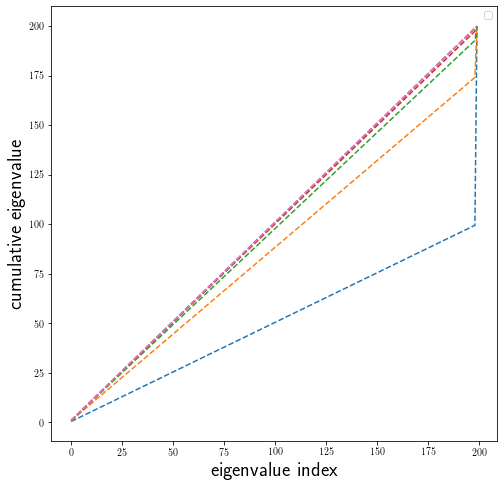
\includegraphics[scale=0.22]{figs/dgn-fra-ecdf-ideal.png}
\end{wrapfigure}
\begin{comment}
\begin{wrapfigure}{h}{0.27\textwidth}
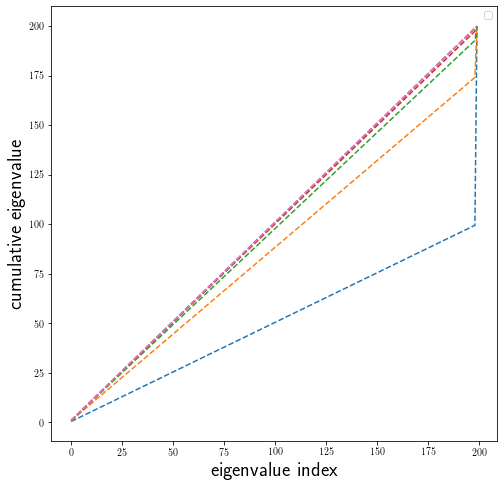
\includegraphics[scale=0.22]{figs/dgn-fra-ecdf-ideal.png}
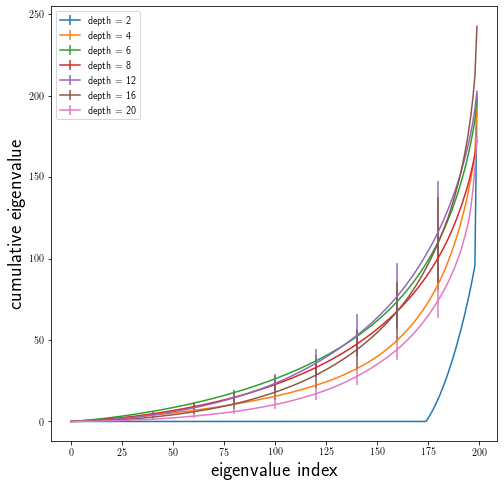
\includegraphics[scale=0.22]{figs/dgn-fra-ecdfbyd-w25.png}
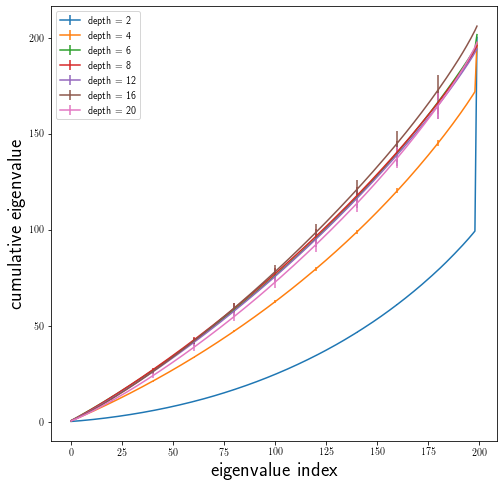
\includegraphics[scale=0.22]{figs/dgn-fra-ecdfbyd-w500.png}
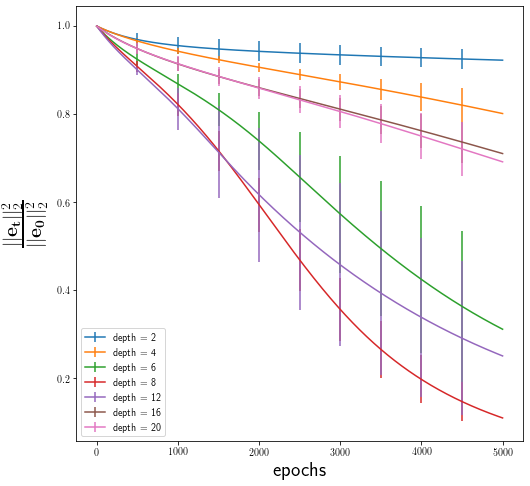
\includegraphics[scale=0.21]{figs/dgn-fra-conv-w25.png}
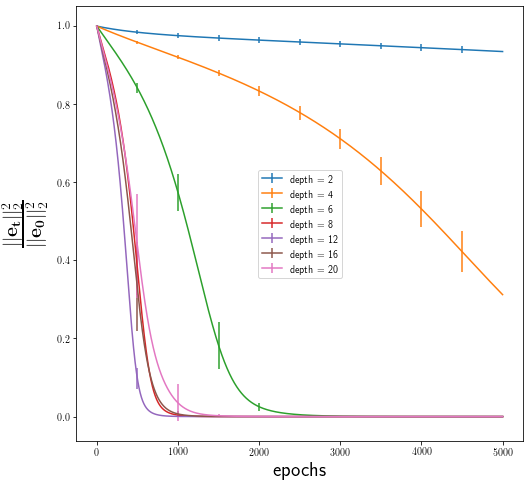
\includegraphics[scale=0.21]{figs/dgn-fra-conv-w500.png}
\caption{}
\label{fig:dgn-frg-gram-ecdf}
\end{wrapfigure}
\end{comment}
We now consider a case where the spectrum of $\lambda_0$ (hence $H_0$ and $K_0$) can be explicitly characterised. Here, for each input example in the dataset, we sample gating values from $Ber(\mu)$ taking values in $\{0,1\}$, and collect it in $\G_0$. In this case, it is easy to check that $\mathbb{E}_{\mu}\left[\lambda_0(s,s)\right]=(\mu w)^{(d-1)},\forall s\in[n]$ and $\mathbb{E}_{\mu}\left[\lambda_0(s,s')\right]=(\mu^2 w)^{(d-1)},\forall s,s'\in[n]$.\\
\textbf{Dataset:} $(x_s,y_s)_{s=1}^n\in \R\times \R$, where $x_s=1,\forall s\in [n]$, and $y_s\sim unif([-1,1])$, $n=200$. \\
\textbf{NPK:} The input Gram matrix $x^\top x$ is a $n\times n$ matrix with all entries equal to $1$ and its rank is equal to 1, and hence $H_0=\lambda_0$.\WFclear
\textbf{Spectrum (Theory):} For $\sigma=\sqrt{\frac{1}{\mu w}}$, and by further averaging $\mathbb{E}_{\mu}\left[K_0(s,s)/d\right]=1$, and $\mathbb{E}_{\mu}\left[K_0(s,s')/d\right]=\mu^{(d-1)}$. Now, let $\rho_i\geq 0,i \in [n]$ be the eigenvalues of $\frac{\E{K_0}}{d}$, and let $\rho_{\max}$ and $\rho_{\min}$ be the largest and smallest eigenvalues. One can easily show that $\rho_{\max}=1+(n-1)\mu^{d-1}$ and corresponds to the eigenvector with all entries as $1$, and $\rho_{\min}=(1-\mu^{d-1})$ repeats $(n-1)$ times, which corresponds to eigenvectors given by $[0, 0, \ldots, \underbrace{1, -1}_{\text{$i$ and $i+1$}}, 0,0,\ldots, 0]^\top \in \R^n$ for $i=1,\ldots,n-1$.\\

\begin{figure}[h]
\resizebox{\textwidth}{!}{
\begin{tabular}{cccc}
%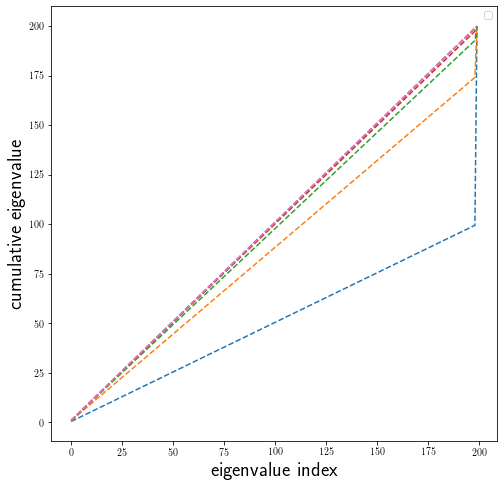
\includegraphics[scale=0.4]{figs/dgn-fra-ecdf-ideal.png}
%&
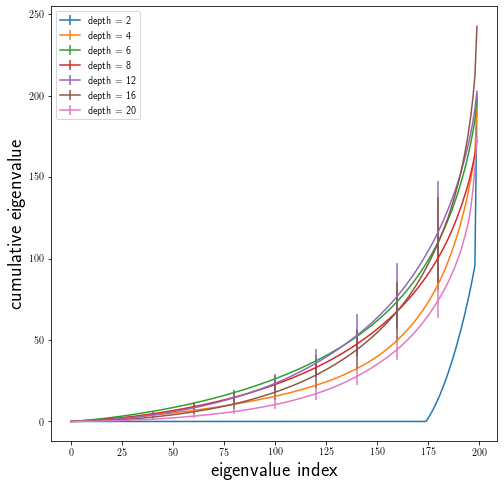
\includegraphics[scale=0.5]{figs/dgn-fra-ecdfbyd-w25.png}
&
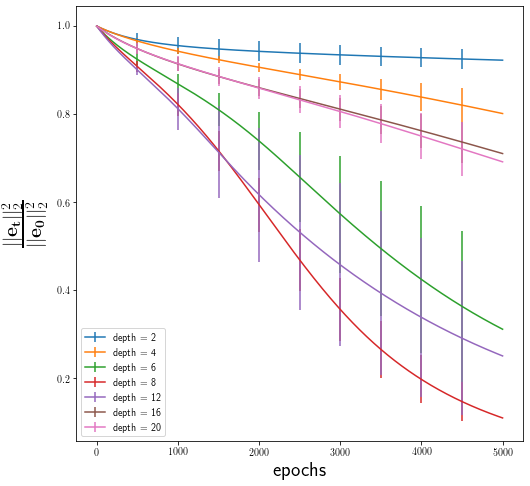
\includegraphics[scale=0.5]{figs/dgn-fra-conv-w25.png}
&
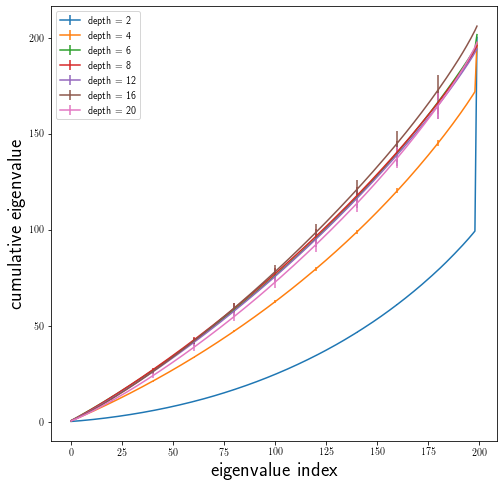
\includegraphics[scale=0.5]{figs/dgn-fra-ecdfbyd-w500.png}
&
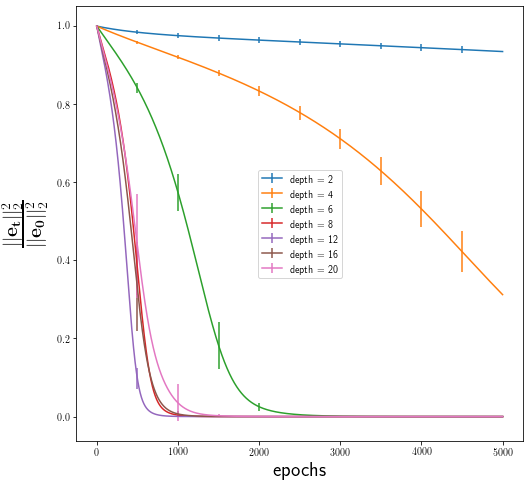
\includegraphics[scale=0.5]{figs/dgn-fra-conv-w500.png}
\end{tabular}
}
\caption{Shows the plots for fixed random gating with $\mu=\frac{1}{2}$ and $\sigma=\sqrt{\frac{2}{w}}$. }
\label{fig:dgn-frg-gram-ecdf}
\end{figure}

\textbf{Spectrum (numerical):} We look at the cumulative eigenvalue (e.c.d.f) obtained by first sorting the eigenvalues in ascending order then looking at their cumulative sum. The ideal behaviour (top plot of \Cref{fig:dgn-frg-gram-ecdf}) as predicted from theory is that for indices $k\in[n-1]$, the e.c.d.f should increase at a linear rate, i.e., the cumulative sum of the first $k$ indices is equal to $k(1-\mu^{d-1})$, and the difference between the last two indices is $1+(n-1)\mu^{d-1}$. In \Cref{fig:dgn-frg-gram-ecdf}, we plot the actual e.c.d.f for various depths $d=2,4,6,8,12,16,20$ and $w=25,500$ a (second and third from top in \Cref{fig:dgn-frg-gram-ecdf}). \hfill\\
\textbf{Convergence (numerical):} In order to compare how the rate of convergence varies with the depth, we set the step-size $\alpha=\frac{0.1}{\rho_{\max}}$, $w=100$. We use the vanilla SGD-optimiser. Note the$ \frac{1}{\rho_{\max}}$ in the stepsize, ensures that the uniformity of maximum eigenvalue across all the instances, and the convergence should be limited by the smaller eigenvalues. We also look at the convergence rate of the ratio $\frac{\norm{e_t}^2_2}{\norm{e_0}^2_2}$. We notice that for $w=25$, increasing depth till $d=8$ improves the convergence, however increasing beyond $d=8$ worsens the convergence rate. For $w=500$, increasing the depth till $d=12$ improves convergence, and $d=16,20$ are worse than $d=12$.  This matches with the depth phenomena observed in practical DNNs and also matches our theory.

\subsection{Generalisation}\label{sec:generalisation}
We trained DGN on standard datasets namely MNIST and CIFAR-10, under the following conditions: i) the gates are fixed $\G_t=\G_0,\forall t\geq 0$ and ii) the gating values are obtained from a ReLU network, which acts as the gating network (see \Cref{tb:dgn}). Since, the gates are fixed, the NPFs are fixed and the (stochastic) GD learns only the path values. We compare the performance of $4$ different NPFs, wherein, the gates are copied from i) from a randomly initialised ReLU network (untrained), ii) from a ReLU network trained with good dataset iii) ReLU network trained on random labels and iv) ReLU network trained on random pixels. Note that the DGN with these fixed (gates) NPFs are trained on the standard dataset with good labels. From the results in \Cref{tb:npfs}, we can conclude that NPFs are learnt during training, i.e., NPFs obtained from trained networks perform better than NPFs obtained at random initialisation.\\
%\FloatBarrier
\begin{table}[!b]
\begin{tabular}{|c|c|c|c|c|c|c|}\hline
&&&&\multicolumn{3}{c|}{NPF (trained)}\\\cline{5-7}
$(w,d)$	&Dataset		&ReLU		&NPF(Un-trained) 		&Good Label		&Random Label 	&Random Pixel\\\hline
$(128,6)$	& MNIST 		& $98.15$ 		&$96$ 		&$98.3$		&$92.6$			&$94.3$\\\hline
$(256,6)$	& MNIST 		& $98.5$ 		&$96.6$ 		&$98.4$		&$92.0$			&$81.1$\\\hline
$(256,10)$	& MNIST 		& $98.4$ 		&$96.2$ 		&$98.2$		&$72.9$			&$80.3$\\\hline
$(256,10)$	& MNIST 		& $98.4$ 		&$96.2$ 		&$98.2$		&$72.9$			&$80.3$\\\hline
\end{tabular}
\caption{Shows the training and generalisation performance of various NPFs.}
\label{tb:npfs}
\end{table}
\textbf{Relation to prior work:} As seen in \Cref{tb:npfs}, we know that, different NPFs give different generalisation performance. In this light, \Cref{th:main} complements the results by \cite{arora2019exact,cao2019generalization}, in that, one can plug-in the NPK in the place of NTK in their generalisation bounds. Further, the gap in the performance of the DNN and the NTK counterparts can be explained by the fact that the NPK is learnt during training (see \Cref{fig:gen} for more evidence).\\
\textbf{NPF learning during training:} We consider ``Binary''-MNIST data set with two classes namely digits $4$ and $7$, with the labels taking values in $\{-1,+1\}$ and squared loss. We trained a standard DNN with ReLU activation ($w=100$, $d=5$). Let $\widehat{H}_t=\frac{1}{trace(H_t)}H_t$ be the normalised NPK matrix. 
\begin{wrapfigure}{h}{0.3\textwidth}
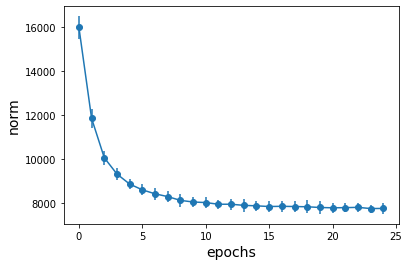
\includegraphics[scale=0.25]{figs/path-gram.png}
\caption{\label{fig:gen}$\nu_t=y^\top (\widehat{H}_t)^{-1} y$.}
\end{wrapfigure}
For a subset size, $n'=200$ ($100$ examples per class) we plot $\nu_t=y^\top (\widehat{H}_t)^{-1} y$, (where $y\in\{-1,1\}^{200}$ is the labeling function), and observe that $\nu_t$ reduces as training proceeds (see \Cref{fig:gen}). Note that, $\nu_t=\sum_{i=1}^{n'}(u_{i,t}^\top y)^2 (\hat{\rho}_{i,t})^{-1}$, where $u_{i,t}\in \R^{n'}$ are the orthonormal eigenvectors of $\widehat{H}_t$ and $\hat{\rho}_{i,t},i\in[n']$ are the corresponding eigenvalues. Since $\sum_{i=1}^{n'}\hat{\rho}_{i,t}=1$, the only way $\nu_t$ reduces is when more and more energy gets concentrated on $\hat{\rho}_{i,t}$s for which $(u_{i,t}^\top y)^2$s are also high.\WFclear%However, in $H_t=(x^\top x)\odot \lambda_t$, only $\lambda_t$ changes with time. Thus, $\lambda_t(s,s')$ which is a measure of overlap of sub-networks active for input examples $s,s'\in[n]$, changes in a manner to reduce $\nu_t$. We can thus infer that the \emph{right} active sub-networks are learned over the course of training.\\s
\textbf{ReLU artefact:}In the case of ReLU activations (i.e., hard gates obtained for $\beta=\infty$ in \Cref{tb:dgn}), the gating values belong to $\{0,1\}$, and it follows that the activity $A_t(\cdot,\cdot)\in\{0,1\}$ and hence $\partial_{\tg} A_t(\cdot,\cdot)=0$. Consequently, there is no flow of the feature gradient in the GD update. However, since the gating parameter $\Tg$ identical with $\Theta$, (i.e., $\Tg_t=\Theta_t,\forall t$), $A_t$ changes with time due to the flow of the value gradient and NPF also changes with time. As a result, understanding feature learning in DNNs with ReLU activations is difficult, and we leave it for future work. In the next section, we study feature learning in parameterised DGNs with soft gates instead.


\section{Feature Learning}
\textbf{Sensitive Sub-Network:} For an input $x\in\R^{d_{in}}$, let $\P^{\S}_{x,t}(\tau_{\S})=\{p\in[P]: |\partial_{\tg} A_t(x,p)|\tau_{\S}\}$ be the set of paths, which have activations whose gradient to any of $\Tg\inrdnet$ is greater than some threshold $\tau>0$. Using the property that the slope of the sigmoid diminishes in the extremities, we note that for appropriate choices of $\tau_{\A}$ (sufficiently close to $1$) and $\tau_{\S}$ (large enough), $\P^{\S}(\tau_{S})\cup \P^{\A}(\tau_{\A})$.
We now take a re-look at the NTF and NTK matrices, and explicitly write down the terms related to feature learning. \hfill\\
$2.$ Let us take the case of classification with cross-entropy loss. Say we have trained till some $T$ epochs with good classification (say close to $100\%$) accuracy. Considering the fact that $\hat{y}_T=\Phi_{\Tg_T}v_{\Theta_T}$, the gradient with respect to $\Tg$ will change the NPF matrix $\Phi_{\Tg_T}$ in such a manner to reduce the loss, i.e., increase the margin of each of the classified examples. We test this hypothesis  of \emph{margin-increase} due to feature learning in the following toy experiment.\hfill\\
\textbf{A Toy Experiment:} We look at a simple neural network with $d_{in}=2$, $w=2$ and $1$-hidden layer (see first diagram on the left in \Cref{fig:feat}). The first layer weights is an identity matrix, and for input $x\in\R^2$ to the network, the first layer output is given by $z_{t}(i)=x(i)G_t(i),i=1,2$, where $G_t(i)=\frac{1}{1+\exp(-\tg(i))},i=1,2$. In this network, there are $2$ paths, and the NPF is given by $\phi_{x,t}=(x(1)G_t(1),x(2)G_t(2))\in \R^2$ (note that this mimics the general structure of the NPF as presented in \Cref{sec:expressivity}).
We check the performance of frozen-gates versus adaptable gates in this network. The dataset is $(x_s,y_s)_{s=1}^{n},n=1000$, wherein, for $s=,1,\ldots,500$, $x_s(1)\stackrel{iid}\sim U[0.1,1]$, and $x_s(2)\stackrel{iid}\sim U[-100,100]$, and $y_s=1$, and for $s=501,\ldots,1000$, $x_s(1)\stackrel{iid}\sim U[-0.1,-1]$, and $x_s(2)\stackrel{iid}\sim U[-100,100]$, and $y_s=-1$. We use the loss function $L_t=\frac{1}{n}\sum_{s=1}^n\frac{1}{1+exp(-y_s\hat{y}_t(x_s))}$. The maximum margin classifier in this case is: predict $+1$ if $x(1)>0$ and else predict $-1$. We trained the simple neural network using gradient descent with step-size of $0.1$, and initialisation $\Tg_0=\Theta_0=(0,0)\in\R^2$ for the following two cases: i) frozen-gates, wherein, we set $\Tg_0=\Tg_t=\Tg_0,\forall t\geq 0$, so that the input features are not transformed, and train only $\Theta_t$ ii) adaptable gates, wherein, we train both $\Tg_t$ and $\Theta_t$. While both cases train for $T=10^4$ epochs, for $T=10^3$ epochs only the model with adaptable gates trains successfully. The results are shown in \Cref{fig:feat}, notice that the right most plot shows that in the case when the gates are adapting, they learn to suppress the second co-ordinate (the scale of $\phi_{x_s,T}$ is from $-15$ to $15$ as opposed to $-100$ to $100$ in $x_s$).
\FloatBarrier
\begin{figure}[h]
\begin{minipage}{0.15\columnwidth}
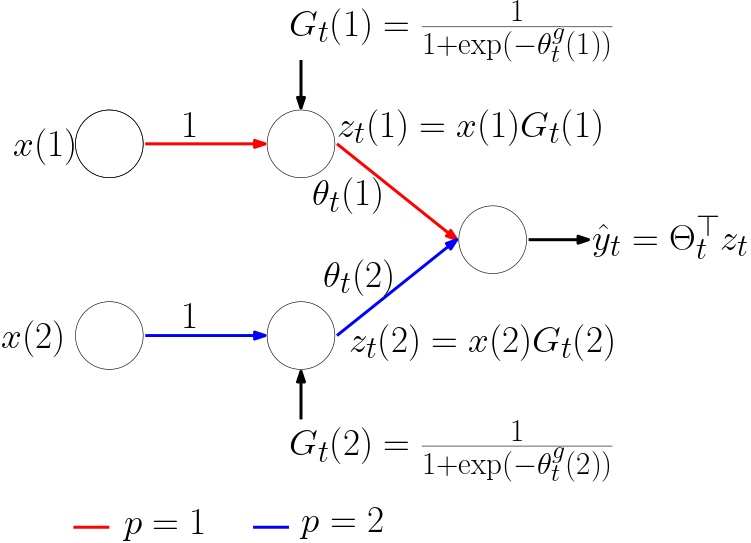
\includegraphics[scale=0.15]{figs/featlearn.png}
\end{minipage}
\hspace{50pt}
\begin{minipage}{0.8\columnwidth}
\resizebox{1\columnwidth}{!}{
\begin{tabular}{cccc}
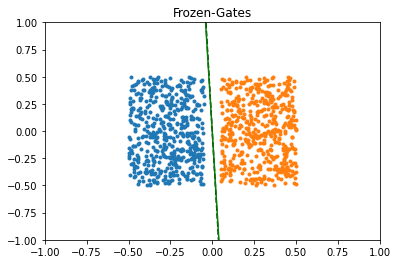
\includegraphics[scale=0.2]{figs/simple-1e2.png}
&
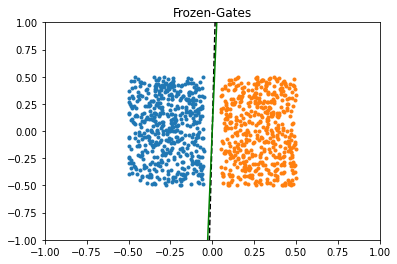
\includegraphics[scale=0.2]{figs/simple-1e3.png}
&
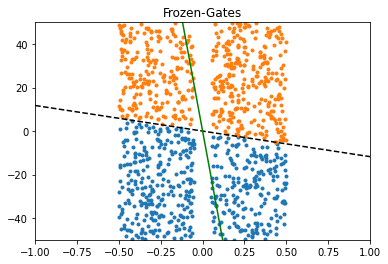
\includegraphics[scale=0.2]{figs/simple.png}
&
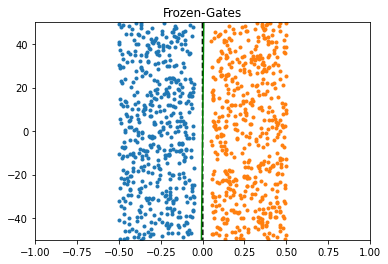
\includegraphics[scale=0.2]{figs/simple-1e4.png}
\\
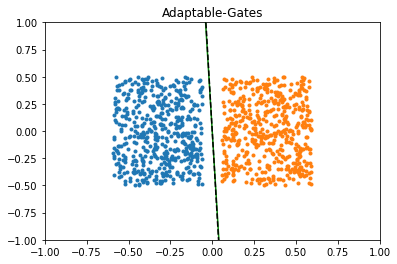
\includegraphics[scale=0.2]{figs/adapt-1e2.png}
&
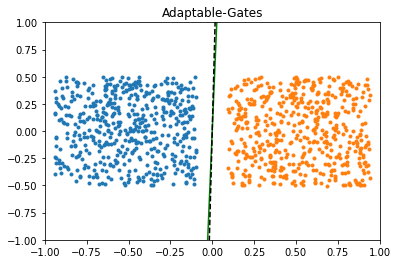
\includegraphics[scale=0.2]{figs/adapt-1e3.png}
&
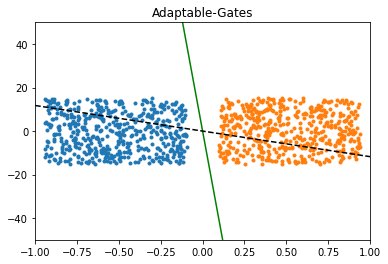
\includegraphics[scale=0.2]{figs/adapt.png}
&
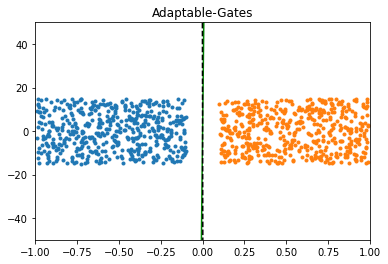
\includegraphics[scale=0.2]{figs/adapt-1e4.png}
\end{tabular}
}
\end{minipage}

\caption{From left: second and third plots shows the training performance of frozen and adaptable gates respectively. In both plots, the bold line in green is the classifier learnt in the case of adaptable gates, and the dotted black line is the classifier learnt in the case of frozen gates. Notice the transformation of the feature space in the case of adaptable gates.}
\label{fig:feat}
\end{figure}
$3.$ \textbf{An open question:} Informally speaking, in the above example, even though the gating parameters had $2$-degrees of freedom, it was nonetheless sufficient to adapt the features. Thus, perhaps we can hypothesise that subject to the `well-conditioned' ness of $K^a_t$, such margin increase can be perhaps achieved for all the $n$ examples.  However, in practice, both $\Tg_t$ as well as $\Theta_t$ change, and an open question is to understand how the joint optimisation and feature learning happens. 
%\section{Conclusion }
\begin{comment}
In this paper, we looked at the gradient descent (GD) procedure to minimise the squared loss in deep neural networks. Prior literature \cite{dudnn} makes trajectory analysis (wherein the dynamics of the error terms are studied) to show that GD achieves zero training error. In this paper, we introduced to important conceptual novelties namely deep gated networks (DGNs) and path-view, to obtain additional insights about GD in the context of trajectory analysis. In particular, our theory threw light on i) the depth phenomena and ii) gate adaptation, i.e., the role played by the dynamics of the gates in generalisation performance.

The path-view lead following gains: (i) an explicit expression of information propagation in DGNs where in the input signal and the wires, i.e., the deep network itself are separated. This is unlike the conventional layer by layer approach, wherein, the input is lost in the hidden layers, (ii) explicitly identifying the role of sub-networks in training and generalisation of deep networks, so much so that, we can go so far as to say that the actual \emph{hidden features are in the paths and the sub-networks and not just the final layer output}, (iii) explicit identification of twin gradient flow, wherein, one component of the gradient flow to train the paths keeping the sub-network constant and the other component of the gradient takes care of learning the gating values.

We looked at various DGNs with adaptable gates and we observed  in experiments that the adaptable/learned gates generalise better than non-adapting/non-learned gates.  Based on our theory and experiments, we conclude that \emph{understanding generalisation would involve a study of gate adaptation}.
\end{comment}
\begin{comment}
In this paper, we introduced to important conceptual novelties namely deep gated networks (DGNs) and path-view, to obtain additional insights about gradient descent in deep learning. The path-view lead to the following gains: (i) an explicit expression of information propagation in DGNs (ii) explicitly identifying the role of sub-networks in training and generalisation of deep networks, (iii) explicit identification of twin gradient flow, wherein, one component of the gradient flow to train the path strengths keeping the sub-network constant and the other component of the gradient takes care of learning the gating values. Using the path-view and the DGNs, we showed  i) the depth helps is equivalent to whitening of data and increasing depth beyond degrades the spectrum of the Gram matrix at initialisation, and ii) gate adaptation, i.e., the role played by the dynamics of the gates is important for generalisation performance.

We looked at various DGNs with adaptable gates and we observed  in experiments that the adaptable/learned gates generalise better than non-adapting/non-learned gates.  Based on our theory and experiments, we conclude that \emph{understanding generalisation would involve a study of gate adaptation}.
\end{comment}

In this paper, we introduced two important conceptual novelties namely deep gated networks (DGNs) and ``path-view", to obtain additional insights about gradient descent in deep learning. Using these two novel concepts, we achieved the following:

 (i) resolution to the depth phenomena for DGNs under decoupling assumption. In particular, our results showed that increasing depth is equivalent to whitening of data and increasing depth beyond a point degrades the spectrum of the Gram matrix at initialisation.
 
 (ii) each input example has a corresponding active sub-network, which are learned when the gates adapt.
 
 (iii) a preliminary theory to analyse gate adaptation. Our analysis points out to the presence of two complementary networks for each input example, one being the active sub-network which holds the memory for that input example and the other being the sensitivity sub-network of gates that are adapting.
 
(iv) we looked at various DGNs with adaptable gates and we observed  in experiments that the adaptable/learned gates generalise better than non-adapting/non-learned gates.  

Based on our theory and experiments, we conclude that :

(a) \emph{Hidden features are in the active sub-networks,} which are in turn decided by the gates.

(b) \emph{Understanding generalisation would involve a study of gate adaptation.}



\begin{comment}
Let $\gamma>0$ be a threshold value, and let $G_{x_s,\Tg_t}(l,i)$ denote the gating value node $i$ in layer $l$. We say that the gate to be \emph{transitioning} for input $s\in[n]$, and weight $\tg(m),m\in[d_{net}]$ if
 \begin{align}
 \left|\frac{\partial G_{x_s,\Tg_t}(l,i)}{\partial \tg(m)}\right|>\gamma,
 \end{align}
 and define a gate to be \emph{flipped} otherwise. Note that,
\begin{align}\label{eq:sensitivepath}
\begin{split}
&\partial_{m}A_{\Tg_t}(x_s,p)=\partial_{m}\Pi_{l=1}^{d-1} G_{x_s,\Tg_t}(l,p(l))\\
&=\sum_{l=1}^{d-1} \partial_{m} G_{x_s,\Tg_t}(l,p(l)) \left(\Pi_{l'\neq l} G_{x_s,\Tg_t}(l',p(l'))\right)
\end{split}
\end{align}

\textbf{Remark:}

i) As $\beta\uparrow\infty$, the soft-ReLU gate resembles the ReLU gate. Thus for a given input example $s$, the gates whose pre-activation inputs have a large absolute value will be close to either $0$ or $1$, and one can always find a high enough $\beta$ such that their sensitivity to $\tg(m)$ is less than $\gamma$.

ii) For an input examples $s,s'\in[n]$, if a path $p$ is active (even for one of the inputs), i.e., $A(x_s,p)\approx 1$, then none of the gates in the path will be sensitive, and hence the magnitude contribution of such as path to the summation in $\delta$ is close to $0$.

iii) For an input examples $s,s'\in[n]$, consider a non-active path, such that all gates close to $1$ except for one of the gates (i.e., the right hand side of \eqref{eq:sensitivepath} is non-zero), which is transitioning. Such paths will make a significant contribution to $\delta$ term. We call the set of such paths the sensitive sub-network.

Based on the above discussion one can say  that a DGN with adaptable gates (which includes standard DNN with ReLU gates), at initialisation, has two kinds of sub-networks for every input example i) the active sub-network comprised of path for which $A(x_s,p)=1$\footnote{or $A(x_s,p)$  is above a given threshold value in the case of soft gates} and ii) the sensitive sub-network which is formed by the set of paths that are sensitive for a given input.
\end{comment}
\bibliographystyle{plainnat}
\bibliography{refs}
\section{Understanding the role of convolutions and pooling operations}\label{sec:conv}
In this section, we will use the frameworks of DGNs and ``path-view'' to obtain insights about (i) convolutional layers and (ii) pooling: global average pooling\footnote{The arguments can be extended to $\max$-pooling with technical modifications.}. In this section, we continue to be in the DGN setup, i.e., we will have separate parameterisations $\Tg$ and $\Tv$, and assume that Assumptions~\ref{assmp:mainone}, \ref{assmp:maintwo} hold. However, we impose additional restrictions to account for the presence of convolutional and pooling layers, which, we describe below.

\textbf{Circular Convolutional layers:}

$1.$ We assume that, the initial $0<L<d$ layers are convolutional layers. In particular, each layer uses a $1$-dimensional kernel of width $0<\hat{w}<d_{in}$, and the output of each layer is a $d_{in}$-dimensional vector.

$2.$ We consider circular convolutional operations instead of zero padding, i.e., during the convolution operation, say index $i$ exceeds $d_{in}$ then it will be considered as $i-d_{in}$, and in the case when a negative index is required, i.e., if index $i<0$ is needed, then $d_{in}+i$ will be used instead. We illustrate this circular convolution with the help of \Cref{fig:circconv}, wherein, $\hat{w}=2$, $d_{in}=3$. Here, $\theta^{(l)}(i),l=1,\ldots,L-1, i=1,2$ are the weights, and the final layer weight $\theta^{(L)}=\left[\frac{1}{d_{in}},\ldots, \frac{1}{d_{in}}\right]^\top\in \R^{d_{in}}$ in the case of global average pooling. Note that, in \Cref{fig:circconv}, we have used only one network, and we have also used a simpler and different notation for the weights: this is because, in DGN (with circular convolutions), both the gating network parameterised by $\Tg$ and the weights network parameterised by $\Tv$ will have identical architecture, and in order to explain just the circular convolution alone more clearly, we have used a simpler notation for the weights and have left the gating information unspecified in \Cref{fig:circconv}.

\begin{figure}
\centering
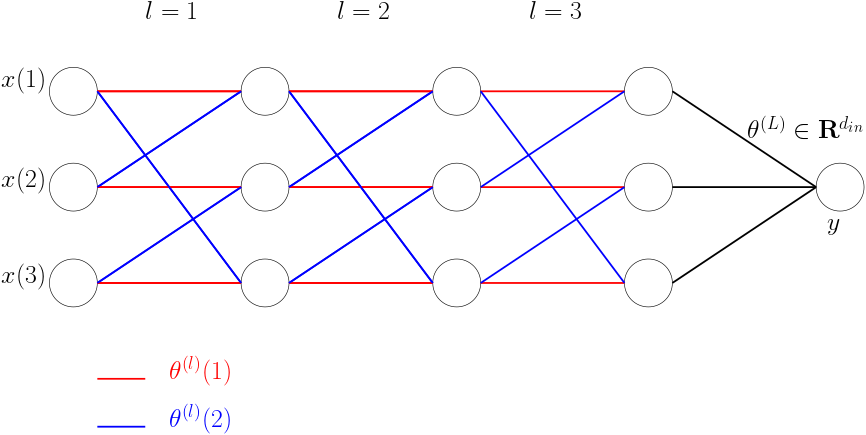
\includegraphics[scale=0.25]{figs/circconv.png}
\caption{Shows a circular convolutional network with $d_{in}=3$ and kernel size $\hat{w}=2$. Note that there are only $8$ unique path strengths in this example (in the case of global average pooling).}
\label{fig:circconv}
\end{figure}



\textbf{Path Sharing:} With the understanding of circular convolution in the background, we now investigate the similarity of two inputs $x_s\in \R^{d_{in}}$ and $x_{s'}\in \R^{d_{in}}$ after they pass through $L$ convolutional layers. To be specific, let $x_s(L)\in \R^{d_in}$ and $x_{s'}(L)\in \R^{d_{in}}$ be the outputs obtained after the $L$ convolutional layers. Note that $x_s(L)=(x_s(L,i),i\in[d_{in}])\in \R^w$ is a $d_{in}$-dimensional vector with $i=1,\ldots,d_{in}$ components, wherein, the $i^{th}$ component is obtained by circular convolution using a kernel of size $0<\hat{w}<d_{in}$. Further, we restrict our attention to the first $L$ layers which perform the convolution operations. We are interested in investigating the following: 
\begin{align}
\E{\ip{x_s(L),x_{s'}(L) }}=\sum_{i=1}^{d_{in}} \E{x_s(L,i)x_{s'}(L,i)}
\end{align}
Given the randomised and symmetric nature of the weight initialisation, without loss of generality, it is sufficient to study $\E{x_s(L,1)x_{s'}(L,1)}$, i.e., it is enough to consider the case of $L$ convolutions with kernel of size $\hat{w}$ followed by a global average pooling. We now make the following observations:

$1.$ There are $p=1,\ldots,\hat{P}=d_{in}\hat{w}^{d-1}$ paths.

$2.$ There are $k=1,\ldots,\hat{B}=\hat{w}^{d-1}$ unique path strengths. This is due to the fact that the same path strength repeats $d_{in}$ times. For instance, in \Cref{fig:circconv}, the path strength $\theta^{1}(1)\theta^{1}(2)\theta^{1}(3)\frac{1}{d_{in}}$ repeats $3$ times.

$3.$ Paths can be grouped into bundles $b_k,k\in[\hat{w}^{d-1}]$, wherein, bundle $b_k$ comprises of $d_{in}$ paths, all of which have the same path strength. Without loss of generality, $b_k$ comprises of paths $(k-1)d_{in}+1,\ldots, kd_{in}$.

$4.$ The path strength $w_t=(w_t(b_1),\ldots, w_t(b_{\hat{B}}))\in \R^{\hat{P}}$, where $w_t(b_k)=(w_t(p),p=(k-1)d_{in}+1,\ldots,kd_{in})\in \R^{d_{in}}$. 

$5.$ The output $x_s(L,1)=\phi^\top_{x_s,\G_t} w_t$.

\begin{lemma}\label{lm:invariance}
At $t=0$, under \Cref{assmp:main}, convolutional layers with global average pooling at the end causes translational invariance.
\begin{align*}
&\E{x_s(L,1)x_{s'}(L,1)}\\&=\frac{\sigma^{2(d-1)}}{d^2_{in}}\sum_{k=1}^{\hat{B}} \sum_{p_1,p_2\in b_k}  \Big( x(p_1(0),s) A(x_s,p_1)\\
&\quad\quad \quad\quad \quad\quad x(p_2(0),s') A(x_{s'},p_2) \Big)
\end{align*}
\end{lemma}

\textbf{Remark:} Now, for $i\in\{0,\ldots, d_{in}-1\}$, let $z^{(i)}\in \R^{d_{in}}$ be the clockwise rotation of $z\in \R^{d_{in}}$ by $i$ co-ordinates, and let $x^{(i)}\in \R^{d_{in}\times n}$ be the data matrix obtained by clockwise rotation of the columns of the data matrix $x\in \R^{d_{in}\times n}$ by $i$ co-ordinates. Then, we have

\begin{align*}
&\E{x_s(L,1)x_{s'}(L,1)}\\
&=\frac{\sigma^{2(d-1)}}{d^2_{in}}\sum_{k=1}^{\hat{B}} \sum_{i=1}^{d_{in}} \sum_{p\in b_k}   \Big(x(p(0),s) A(x,p) \\ 
&\quad\quad \quad\quad \quad\quad x^{(i)}(p(0),s') A(x^{(i)}_{s'},p) \Big)
\end{align*}
The term $\sum_{p\in b_k}  x(p(0),s) A(x,p) x^{(i)}(p(0),s') A(x^{(i)}_{s'},p)$ is translation invariant.


\begin{comment}
\textbf{Claim $2$:} At $t=0$, under Assumptions~\ref{assmp:mainone},\ref{assmp:maintwo}, convolutional layers with $\max$-pooling at the end causes translational invariance.

\begin{proof}
The proof follows in a manner similar to \textbf{Claim $1$} made for the case of global average pooling. However, the technical challenge is the following: in the case of $\max$-pooling, only one of the $d_{in}$ paths connecting the $(L-1)^{th}$ layer to the output node is \emph{on}. This path connects the ``$\max$" node in the $(L-1)^{th}$ layer to the output node. This can be accounted in the calculations by setting the path strength to be $0$ for those paths that do not pass through the ``$\max$" node in the $(L-1)^{th}$ layer.  We make the following observations about $M$:

$1.$ For each bundle $b_k, k\in[\hat{B}]$, $\exists$ unique indices $i(k), j(k)\in [d_{in}]$ such that $M((k-1)d_{in}+i(k), (k-1)d_{in}+j(k))=\sigma^{2(d-1)}$, and rest of the entries of $M$ are $0$.

$2.$ $M(p_1,p_2)=\frac{\sigma^{2(d-1)}}{d^2_{in}}$, if $p_1$ and $p_2$ belong to the same bundle continues to hold trivially due to observation $1$ (of the current claim).

And by going through reductions similar to \textbf{Claim $1$}, we have

\begin{align*}
&\E{x_s(L,1)x_{s'}(L,1)}\\&=\phi^\top_{x_s,\G_0} M \phi^\top_{x_{s'},\G_0}\\
&=\sum_{p_1,p_2=1}^{\hat{P}} \Big(x(p_1(0),s) A(x_s,p_1) \\
&\quad\quad \quad\quad \quad\quad x(p_2(0),s') A(x_{s'},p_2) M(p_1,p_2)\Big)\\
&=\frac{\sigma^{2(d-1)}}\sum_{k=1}^{\hat{B}} \sum_{p_1,p_2\in b_k}  \Big( x(p_1(0),s) A(x_s,p_1)\\
&\quad\quad \quad\quad \quad\quad x(p_2(0),s') A(x_{s'},p_2) \Big)
\end{align*}
Now, for $i\in\{0,\ldots, d_{in}-1\}$, let $z^{(i)}\in \R^{d_{in}}$ be the clockwise rotation of $z\in \R^{d_{in}}$ by $i$ co-ordinates, and let $x^{(i)}\in \R^{d_{in}\times n}$ be the data matrix obtained by clockwise rotation of the columns of the data matrix $x\in \R^{d_{in}\times n}$ by $i$ co-ordinates. Then, we have

\begin{align*}
&\E{x_s(L,1)x_{s'}(L,1)}\\
&=\frac{\sigma^{2(d-1)}}{d^2_{in}}\sum_{k=1}^{\hat{B}} \sum_{i=1}^{d_{in}} \sum_{p\in b_k}   \Big(x(p(0),s) A(x,p) \\ 
&\quad\quad \quad\quad \quad\quad x^{(i)}(p(0),s') A(x^{(i)}_{s'},p) \Big)
\end{align*}
The term $\sum_{p\in b_k}  x(p(0),s) A(x,p) x^{(i)}(p(0),s') A(x^{(i)}_{s'},p)$ is translation invariant.

\end{proof}
\end{comment}
\section{Proofs}


%
\onecolumn
\begin{center}
Appendix/Supplementary Material
\end{center}
\section{Paths}\label{sec:path}
%\subsection{Zeroth Order Terms}
\textbf{Vectorised Notation:} Given a dataset $(x_s,y_s)_{s=1}^n\in \R^{d_{in}}\times \R$, let data be represented as matrices $x\in\R^{d_{in}\times n}$ and $y\in \R^n$ with the convention that $x_s=x(\cdot,s)\in\R^{d_{in}}$ and $y_s=y(s)\in \R$. For the purpose of this section we follow the vectorised notation in \Cref{tb:dgnvector}.

\FloatBarrier
\begin{table}[h]
\centering
\begin{tabular}{|c|c|}\hline
Input layer & $x(s,i,0) =x(i,s)$ \\\hline
Pre-activation& $q_t(s,i,l)= {\Theta_t(l,\cdot,i)}^\top x_t(s,\cdot,l-1) $ \\\hline
Layer output & $x_t(s,i,l)= q_t(s,i,l) G_t(s,i,l)$ \\\hline
Final output & $\hat{y}_t(x)={\Theta_t(d,\cdot,1)}^\top x_t(s,\cdot,d-1)$\\\hline
\end{tabular}
\caption{A deep gated network in the vectorised form. $l=1,\ldots,d-1$ denote the intermediate layers.}
\label{tb:dgnvector}
\end{table}




The idea behind the ``path view'' is to regard the given neural network as multitude of connections from input to output.  We now describe the zeroth and first order terms in the language of paths.
\begin{definition}[Neural Path]
Let $\P=[d_{in}]\times [w]^{d-1}$ be a cross product of index sets. Define a path $p$ by $p\stackrel{def}=(p(0),p(1),\ldots,p(d-1))\in \P$, where $p(0)\in [d_{in}]$, and $p(l)\in[w],\forall l\in[d-1]$. 
\end{definition}

A path $p$ starts at an input node $p(0)$ goes through nodes $p(l)$ in layer $l\in[d-1]$ and finishes at the output node .%(see \Cref{fig:path}%\todoch{Need to add a diagram like the recent lottery ticket weight Vivek Ramanujam paper.}). 
%In what follows, we use $p\rsa (\cdot)$ to denote the fact that path $p$ passes through node $(\cdot)$, where $(\cdot)$ is an input node, or a weight in some layer, or a hidden node.

\begin{definition}\label{def:strength}[Strength]
Each path is also associated with a strength given by: $w_t(p)=\Pi_{l=1}^d \Theta_t(l,p(l-1),p(l))$
%\begin{align}
%$w_t(p)=\Pi_{l=1}^d \Theta_t(l,p(l-1),p(l))$
%\end{align}
\end{definition}

\begin{definition}\label{def:activity}[Activation Level]
The activity of a path $p$ for input $s$ is given by: $A(s,p)=\Pi_{l=1}^d G(s,p(l),l)$
%\begin{align}
%$A(s,p)=\Pi_{l=1}^d G(s,p(l),l)$
%\end{align}
\end{definition}
In the case when $G\in \{0,1\}$ it also implies that $A\in \{0,1\}$.  %Thus $A(s,p)$ tells us whether the path $p$ is \emph{active} when $s^{th}$ input example is presented to the network.

\begin{definition}\label{def:feature}[Neural Feature]
Given a gating pattern $\G_t$, define 
\begin{align}
\phi_{x_s,\G_t}(p)\stackrel{def}=x(p(0),s) A_{\G_t}(x_s,p),
\end{align}
and let $\phi_{x_s,\G_t}=(\phi_{x_s\G_t}(p),p\in [P])\in \R^P$ be the hidden feature corresponding to input $x_s$. Let $\Phi_{x,\G_t}=\left[\phi_{x_1,\G_t}| \ldots |\phi_{x_n,\G_t}\right]\in \R^{P\times n}$ be the feature matrix obtained by stacking the features $\phi_{x_s,\G_t}$ of inputs $x_s\in \R^{d_{in}}$ column-wise.
\end{definition}

\comment{
\textbf{Predicted} output of the network is given in terms of the paths by $\hat{y}_{t}(s)=\sum_{p\in P} x(p(0),s) A_{\G_t}(x_s,p) w_t(p)$, i.e., 
\begin{align}\label{eq:zeroth}
\hat{y}_{t}(s)=\Phi_{x,\G_t}^\top w_{t}
\end{align}

%\begin{figure}
%\centering
%\includegraphics[scale=0.2]{mickey.png}
%\caption{Some picture to break the monotony}
%\end{figure}

%\textbf{Sub-networks:} %An important fact that can be seen as an immediately from the path based representation is that DGNs 
\textbf{Sub-networks:}  In DGNs similarity of two different inputs $x_s,x_{s'}\in \R^{d_{in}}, s,s' \in [n]$ depends on the overlap of path that are \emph{active} for both inputs. This can be seen by noting that $\phi_{x_s,\G_t}^\top \phi_{x_s,\G_t}=\sum_{i=1}^{d_{in}} x(i,s)x(i,s') \underset{p\rsa i}{\sum} A_{\G_t}(x_s,p) A_{\G_t}(x_{s'},p)$. Consider for instance a DGN whose gating values are in $\{0,1\}$, and say $n=2$, i.e., the dataset contains only two inputs $x_1,x_2\in \R^{d_{in}}$. From \eqref{eq:pathsim} it is clear that if inputs $x_1,x_2$ do not share any common \emph{active} paths throughout training, then they are \emph{orthogonal} to each other, because $A_{\G_t}(s,p) A_{\G_t}(s',p)=0, \forall p\in [P]$. This makes intuitive sense because in this case, it is as though there are two parallel networks (while the weights can be shared, the paths are not). Thus it is clear from the path based representation in \eqref{eq:zeroth} and \eqref{eq:pathsim}, the gating pattern $\G_t$ plays are crucial role in DGNs via the activation levels $A_{\G_t}(\cdot,\cdot)$.
%\subsection{First Order Terms}
The feature $\phi_{x_s,\G_t}$ in \Cref{def:feature} as well as the strength $w_t$ in \Cref{def:strength} are $P$-dimensional quantities. However, loosely speaking, the DGN has only as much \emph{degrees of freedom} as the number of trainable parameters (which we denote by $d_{net}$). 
\begin{definition}[Neural Tangent Features] The  $d_{net}\times n$ NTF matrix is defined as $\Psi_t(m,s)\stackrel{def}=\frac{\partial \hat{y}_{t}(x_s)}{\partial \theta(m)},m\in [d_{net}], s\in [n]$. 
\comment{
\begin{align}\label{eq:split}
\begin{split}
&\Psi_t(m,s) = \frac{\partial \hat{y}_t(x_s)}{\partial \theta(m)}\\
&=\frac{\partial }{\partial \theta(m)}\left(\sum_{p\in P} x(p(0),s) w_{t}(p) A_{\G_t}(s,p)\right),\\
&=\underbrace{\left(\sum_{p\in P} x(p(0),s) \frac{\partial w_{t}(p)}{\partial \theta(m)} A_{\G_t}(s,p)\right)}_{\text{sensitivity of strength}}\\
&\quad\quad\quad\quad\quad\quad\quad\quad+\\
&=\underbrace{\left(\sum_{p\in P} x(p(0),s) w_{t}(p) \frac{\partial A_{\G_t}(s,p)}{\partial \theta(m)}\right)}_{\text{sensitivity of activations}}
\end{split}
\end{align}

\begin{align}\label{eq:split}
\begin{split}
&\Psi_t(m,s) = \frac{\partial \hat{y}_t(x_s)}{\partial \theta(m)}\\
&=\frac{\partial }{\partial \theta(m)}\left(\sum_{p\in P} x(p(0),s) w_{t}(p) A_{\G_t}(s,p)\right),\\
&=\underbrace{\left(\sum_{p\in P} x(p(0),s) \frac{\partial w_{t}(p)}{\partial \theta(m)} A_{\G_t}(s,p)\right)}_{{\Psi^w_{t}(m,s)}}\\
&\quad\quad\quad\quad\quad\quad\quad\quad+\\
&=\underbrace{\left(\sum_{p\in P} x(p(0),s) w_{t}(p) \frac{\partial A_{\G_t}(s,p)}{\partial \theta(m)}\right)}_{{\Psi^a_t(m,s)}}
\end{split}
\end{align}
}
\comment{
\begin{align}\label{eq:split}
\begin{split}
\Psi_t(m,s) &= \underbrace{\left(\sum_{p\in P} x(p(0),s) \frac{\partial w_{t}(p)}{\partial \theta(m)} A_{\G_t}(s,p)\right)}_{{\Psi^w_{t}(m,s)}}\\
&\quad\quad\quad\quad\quad\quad\quad\quad+\\
&=\underbrace{\left(\sum_{p\in P} x(p(0),s) w_{t}(p) \frac{\partial A_{\G_t}(s,p)}{\partial \theta(m)}\right)}_{{\Psi^a_t(m,s)}}
\end{split}
}
\begin{align}\label{eq:split}
\begin{split}
\Psi_t(m,s) &= \Psi^w_{t}(m,s)+\Psi^a_{t}(m,s), \,\text{where}\\
\Psi^w_{t}(m,s)&={\left(\sum_{p\in P} x(p(0),s) \frac{\partial w_{t}(p)}{\partial \theta(m)} A_{\G_t}(s,p)\right)}\\
\Psi^a_{t}(m,s)&={\left(\sum_{p\in P} x(p(0),s) w_{t}(p) \frac{\partial A_{\G_t}(s,p)}{\partial \theta(m)}\right)}
\end{split}
\end{align}


\end{definition}

\textbf{Strength and Gate adaptation:} From \eqref{eq:split} it is clear that there are two \emph{atomic} components to the gradient of the output $\hat{y}_t(x_s)$ with respect to any trainable weight $\theta(m), m=1,\ldots, d_{net}$, namely \emph{neural tangent feature of strength} denoted by $\Psi^w_{t}\in \R^{d_{net}\times n}$ and \emph{neural tangent feature of activations} denoted by $\Psi^a_{t}\in \R^{d_{net}\times n}$. %Before we separately define these two \emph{atomic} components, we would like to mention that as a result of the $\frac{\partial A_{\G_t}(s,p)}{\partial \theta(m)}$ term, gates adapt all throughout training, which in turn affect the output (see \eqref{eq:zeroth}) via $A_{\G_t}$.

}


\comment{
\begin{definition}[Neural Tangent Features of Path Activations (NTFPA)]
\begin{align}
\varphi^a_{t,p}\stackrel{def}{=}\left(\frac{\partial w_{t}(p)}{\partial \theta(m)},m\in[d_{net}]\right)\in \R^{d_{net}},
\end{align}
\end{definition}

\begin{remark}
Let $\theta(m)$ belong to layer $l'\in [d-1]$, then 
\begin{align*}
\varphi^a_{t,p}(m)&=0, \forall p\bcancel{\rsa}\theta(m)
\end{align*}
\end{remark}

Using the sensitivity of strengths and activations at the level of resolution of paths, we now define the neural tangent feature (NTF) for the strengths and activations.

\begin{definition}\label{def:ntf}[Neural Tangent Features]
\begin{align}
\begin{split}
\Psi^w_t(m,s) &=\left(\sum_{p\in P} x(p(0),s) \frac{\partial w_{t}(p)}{\partial \theta(m)} A_{\G_t}(s,p)\right)\\
\Psi^a_t(m,s) &=\left(\sum_{p\in P} x(p(0),s) w_{t}(p) \frac{\partial A_{\G_t}(s,p)}{\partial \theta(m)}\right)\\
\Psi_t(m,s)&=\Psi^w_t(m,s)+ \Psi^a_t(m,s)
\end{split}
\end{align}
\end{definition}


\begin{definition}[Interaction Coefficient]
\begin{align*}
&\lambda^{s,s'}_t(i)\stackrel{def}=\underset{p_1,p_2\rsa\theta(m),i}{\sum_{p_1,p_2\in P:}}  \varphi_{t,p_1}(m)A(s,p_1)  \varphi_{t,p_2}(m) A(s',p_2)
\end{align*}
\end{definition}

\begin{lemma}
\begin{align*}
{K^w_t(s,s')}=\sum_{i=1}^{d_{in}} x(i,s)x(i,s') \lambda^{s,s'}_t(i)
\end{align*}
\end{lemma}

\begin{assumption}\label{assmp:main}\hfill
\begin{enumerate}
\item $\G_0$ is statistically independent of $\Theta_0$.
\item $\Theta_0\stackrel{iid}\sim Ber(\frac{1}{2})$ over the set $\{-\sigma,+\sigma\}$. 
\end{enumerate}
\end{assumption}

\textbf{Remarks on Assumption~\ref{assmp:main}}
In a standard DNN with ReLU activations, the activations and weights are not statistically independent because conditioned on the fact that a ReLU is \emph{on}, the incoming edges cannot be simultaneously all $-\sigma$. We side step this issue by the first condition in Assumption~\ref{assmp:main}, wherein, we assume that  gating is statistically independent of the weights $\Theta_0$. This clears the way to carry out the algebra of paths, which can be boiled down in simple words as the effect on weights in the direction of one path does not affect the contribution of any other path in expectation. This is captured in Lemma~\ref{lm:pathdot} below.
\begin{figure}
\centering
\includegraphics[scale=0.2]{mickey.png}
\caption{Shows that the incoming weights of a ReLU gate which are \emph{on} are not symmetrically distributed.}
\end{figure}

\begin{lemma}\label{lm:pathdot}
Let $\theta(m)$ be an arbitrary weight in layer $l'\in [d-1]$, under Assumption~\ref{assmp:init} we have for paths $p,p_1,p_2\rsa\theta(m), p_1\neq p_2$
\begin{align*}
\E{\varphi_{\Tb,p_1}(m)\varphi_{\Tb,p_2}(m)}= &0\\
\E{\varphi_{\Tb,p}(m)\varphi_{\Tb,p}(m)}= &\left(\frac{2\sigma^2}{w}\right)^{d-1}
\end{align*}
\end{lemma}
\begin{proof}
If $\theta$
Note that $\varphi_{\Tb,p}=\underset{l\neq l'}{\underset{l=1}{\overset{d}{\Pi}}} \Tb(l,p(l-1),p(l))$. Hence
\begin{align*}
&\E{\varphi_{\Tb,p_1}(m)\varphi_{\Tb,p_2}(m)}\\
&=\E{\underset{l\neq l'}{\underset{l=1}{\overset{d}{\Pi}}} \Bigg(\Tb(l,p_1(l-1),p_1(l))\Tb(l,p_2(l-1),p_2(l)) \Bigg)}\\
&=\underset{l\neq l'}{\underset{l=1}{\overset{d}{\Pi}}}\E{\Tb(l,p_1(l-1),p_1(l))\Tb(l,p_2(l-1),p_2(l))}
\end{align*}

Since $p_1\neq p_2$, in one of the layers $\tilde{l}\in[d-1],\tilde{l}\neq l'$ they do not pass through the same weight. Using this fact
\begin{align*}
&\E{\varphi_{\Tb,p_1}(m)\varphi_{\Tb,p_2}(m)}\\
&=\left(\underset{l\neq l',\tilde{l}}{\underset{l=1}{\overset{d}{\Pi}}}\E{\Tb(l,p_1(l-1),p_1(l))\Tb(l,p_2(l-1),p_2(l))}\right)\\
&\Bigg(\E{\Tb(\tilde{l},p_1(\tilde{l}-1),p_1(\tilde{l}))}\E{\Tb(\tilde{l},p_2(\tilde{l}-1),p_2(\tilde{l}))}\Bigg)\\
&=0
\end{align*}
\end{proof}


\begin{definition}[Path Similarity]
\begin{align*}
\mu^{s,s'}(i)=\sum_{m=1}^{d_{net}} \underset{p\rsa\theta(m)}{\sum_{p\in P: p(0)=i}}A(s,p) A(s',p)
\end{align*}

\end{definition}

\begin{lemma}
\begin{align*}
\mathbf{E}_{\Theta_0}\left[\lambda^{s,s'}_0(i)\right]=\sigma^{2(d-1)}\mu^{s,s'}(i)
\end{align*}
\end{lemma}

\begin{theorem}\label{th:dgnexp}
 Under Assumption~\ref{assmp:main}
 \begin{align*}
\mathbf{E}_{\Theta_0}\left[K_0(s,s')\right]=\sigma^{2(d-1)}\sum_{i=1}^{d_{in}}x(i,s) x(i,s')\mu^{s,s'}(i)
\end{align*}

\end{theorem}
\begin{proof}
See Appendix.
\end{proof}

\begin{theorem}\label{th:dgnvar}
 Under Assumption~\ref{assmp:main} $Var\left[K_0\right]\leq $
\end{theorem}

}
% This document was modified from the file originally made available by
% Pat Langley and Andrea Danyluk for ICML-2K. This version was created
% by Iain Murray in 2018, and modified by Alexandre Bouchard in
% 2019. Previous contributors include Dan Roy, Lise Getoor and Tobias
% Scheffer, which was slightly modified from the 2010 version by
% Thorsten Joachims & Johannes Fuernkranz, slightly modified from the
% 2009 version by Kiri Wagstaff and Sam Roweis's 2008 version, which is
% slightly modified from Prasad Tadepalli's 2007 version which is a
% lightly changed version of the previous year's version by Andrew
% Moore, which was in turn edited from those of Kristian Kersting and
% Codrina Lauth. Alex Smola contributed to the algorithmic style files.

\subsection{Results in \Cref{sec:optimisation}}
\textbf{Stament and Proof of Lemma~\ref{lm:sigwire}}
\begin{lemma}[Signal vs Wire Decomposition]
Let $\kappa_t(s,s',i)\stackrel{def}=\underset{p_1,p_2\rsa i}{\sum_{p_1,p_2\in P:}} A_{\G_t}(x_s,p_1) A_{\G_t}(x_{s'},p_2) \ip{\varphi_{t,p_1}, \varphi_{t,p_2}}$. The Gram matrix $K_t$ is then given by 
\begin{align}\label{eq:ktalg}
{K_t(s,s')}=\sum_{i=1}^{d_{in}} x(i,s)x(i,s') \kappa_t(s,s',i)
\end{align}
\end{lemma}

\begin{proof}
Note that
\begin{align*}
\hat{y}_{t}(x_s)=\sum_{p\in\P}x(p(0),s) A(x_s,p) w_t(p)
\end{align*}
Differentiating with respect to any of the weights $\theta(m),m\in[d_{net}]$, we have
\begin{align*}
\frac{\partial \hat{y}_{t}(x_s)}{\partial \theta(m)}&=\frac{\partial \sum_{p\in\P}x(p(0),s) A(x_s,p) w_t(p)}{\partial \theta(m)}\\
\Psi_t(m,s)&=\sum_{p\in\P}x(p(0),s) A(x_s,p) \frac{\partial w_t(p)}{\partial \theta(m)}\\
&=\sum_{p\in\P}x(p(0),s) A(x_s,p) \varphi_{t,p}(m)
\end{align*}

Since, only the path strengths are changing, the Gram matrix $K_t$ is given by 
\begin{align*}
K_t(s,s')&={\Psi_t(\cdot,s)}^\top \Psi_t(\cdot,s')\\
&=\sum_{m=1}^{d_{net}} \Psi_t(m,s) \Psi_t(m,s')\\
&=\sum_{m=1}^{d_{net}} \left(\sum_{p_1\in\P}x(p_1(0),s) A(x_s,p_1) \varphi_{t,p_1}(m)\right)\left(\sum_{p_2\in\P}x(p_2(0),s') A(x_{s'},p_2) \varphi_{t,p_2}(m)\right)\\
&=\sum_{m=1}^{d_{net}} \underset{p_1,p_2\rsa\theta(m)}{\sum_{p_1,p_2\in P:}} x(p_1(0),s) A(x_s,p_1)x(p_2(0),s') A(x_{s'},p_2) \varphi_{t,p_1}(m) \varphi_{t,p_2}(m)\\
&=\sum_{i=1}^{d_{in}}\underset{p_1,p_2\rsa i}{\sum_{p_1,p_2\in P:}} x(p_1(0),s) A(x_s,p_1)x(p_2(0),s') A(x_{s'},p_2) \ip{\varphi_{t,p_1}, \varphi_{t,p_2}}\\
&=\sum_{i=1}^{d_{in}}\underset{p_1,p_2\rsa i}{\sum_{p_1,p_2\in P:}} x(i,s) A(x_s,p_1)x(i,s') A(x_{s'},p_2) \ip{\varphi_{t,p_1}, \varphi_{t,p_2}}\\
&=\sum_{i=1}^{d_{in}} x(i,s)x(i,s') \underset{p_1,p_2\rsa i}{\sum_{p_1,p_2\in P:}} A(x_s,p_1) A(x_{s'},p_2) \ip{\varphi_{t,p_1}, \varphi_{t,p_2}}
\end{align*}
\end{proof}


\textbf{Statement and Proof of Lemma~\ref{lm:pathdot}}
\begin{lemma}
Under Assumption~\ref{assmp:mainone}, for paths $p,p_1,p_2\in \P, p_1\neq p_2$, at initialisation we have (i) $\E{\ip{\varphi_{0,p_1}, \varphi_{0,p_2}}}= 0$, (ii) ${\ip{\varphi_{0,p}, \varphi_{0,p}}}= d\sigma^{2(d-1)}$
\end{lemma}

\begin{proof}
\begin{align*}
\ip{\varphi_{t,p_1}, \varphi_{t,p_2}}= \sum_{m=1}^{d_{net}} \varphi_{t,p_1}(m)\varphi_{t,p_2}(m)
\end{align*}
Let $\theta(m),m\in[d_{net}]$ be any weight such that $p\rsa \theta(m)$, and w.l.o.g let $\theta(m)$ belong to layer $l'\in[d]$. 
If either $p_1\bcancel{\rsa}\theta(m)$ or $p_2\bcancel{\rsa}\theta(m)$, then it follows that $\varphi_{t,p_1}(m)\varphi_{t,p_2}(m)=0$. In the case when $p_1,p_2\rsa\theta(m)$, we have
\begin{align*}
&\E{\varphi_{0,p_1}(m)\varphi_{0,p_2}(m)}\\
&=\E{\underset{l\neq l'}{\underset{l=1}{\overset{d}{\Pi}}} \Bigg(\Tb_0(l,p_1(l-1),p_1(l))\Tb_0(l,p_2(l-1),p_2(l)) \Bigg)}\\
&=\underset{l\neq l'}{\underset{l=1}{\overset{d}{\Pi}}}\E{\Tb_0(l,p_1(l-1),p_1(l))\Tb_0(l,p_2(l-1),p_2(l))}
\end{align*}
where the $\E{\cdot}$ moved inside the product because at initialisation the weights (of different layers) are independent of each other.
Since $p_1\neq p_2$, in one of the layers $\tilde{l}\in[d-1],\tilde{l}\neq l'$ they do not pass through the same weight, i.e., $\Tb_0(\tilde{l},p_1(\tilde{l}-1),p_1(\tilde{l}))$ and $\Tb_0(\tilde{l},p_2(\tilde{l}-1),p_2(\tilde{l}))$ are distinct weights. Using this fact
\begin{align*}
&\E{\varphi_{0,p_1}(m)\varphi_{0,p_2}(m)}\\
&=\underset{l\neq l',\tilde{l}}{\underset{l=1}{\overset{d}{\Pi}}}\E{\Tb_0(l,p_1(l-1),p_1(l))\Tb_0(l,p_2(l-1),p_2(l))}\\
&=\E{\Tb_0(\tilde{l},p_1(\tilde{l}-1),p_1(\tilde{l}))}\E{\Tb_0(\tilde{l},p_2(\tilde{l}-1),p_2(\tilde{l}))}\\
&=0
\end{align*}

The proof of (ii) is complete by noting that $\sum_{m=1}^{d_{net}} \varphi_{t,p}(m)\varphi_{t,p}(m)$ has $d$ non-zero terms for a single path $p$ and at initialisation we have 
\begin{align*}
&{\varphi_{0,p}(m)\varphi_{0,p}(m)}\\
&={\underset{l\neq l'}{\underset{l=1}{\overset{d}{\Pi}}} \Tb^2_0(l,p(l-1),p(l))}\\
&=\sigma^{2(d-1)}
\end{align*}
\end{proof}

\textbf{Statement and Proof of Theorem~\ref{th:dgnexp}}
\begin{theorem}[DIP in DGN]
Under Assumption~\ref{assmp:mainone}, ~\ref{assmp:maintwo}, and $\frac{4d}{w^2}<1$ it follows that
 \begin{align*}
&\E{K_0}=d\sigma^{2(d-1)}(x^\top x \odot \lambda_0)\\
&Var\left[K_0\right]\leq O\left(d^2_{in}\sigma^{4(d-1)}\max\{d^2w^{2(d-2)+1}, d^3w^{2(d-2)}\}\right)
\end{align*}
\end{theorem}

\begin{proof}
The first of the above two claims follow from the algebraic expression for $K_t$ and Lemma~\ref{lm:pathdot}. We now look at the variance calculation. The idea is that we expand  $Var\left[K_0(s,s')\right]=\E{K_0(s,s')^2} -\E{K_0(s,s')}^2$ and identify the the terms which cancel due to subtraction and then bound the rest of the terms.% Further, in what follows, we will assume $d_{in}=1$ without loss of generality.

Let $\theta(m)$ belong to layer $l'(m)$, then 
\begin{align}\label{eq:kexpect}
\E{K_0(s,s')}&=\sum_{m=1}^{d_{net}}\E{\left(\sum_{p_1 \in P}x(p_1(0),s)A(s,p_1)\frac{\partial w_{\Tb}(p_1)}{\partial \theta(m)}\right)\left(\sum_{p_2\in P}x(p_2(0),s)A(s',p_2)\frac{\partial w_{\Tb}(p_2)}{\partial \theta(m)}\right)}\nn\\
&=\sum_{m=1}^{d_{net}}\E{\sum_{p_1,p_2\in P}x(p_1(0),s)A(s,p_1)\frac{\partial w_{\Tb}(p_1)}{\partial \theta(m)}x(p_2(0),s')A(s',p_2)\frac{\partial w_{\Tb}(p_2)}{\partial \theta(m)}}\nn\\
&=\sum_{m=1}^{d_{net}}\underset{p_1,p_2\rsa\theta(m)}{\sum_{p_1,p_2\in P}}x(p_1(0),s)A(s,p_1)x(p_2(0),s')A(s',p_2) \E{\underset{l\neq l'(m)}{\underset{l=1}{\overset{d-1}{\Pi}}} \Tb_0(l,p_1(l-1),p_1(l)) \Tb_0(l,p_2(l-1),p_2(l))}\nn\\
&\stackrel{(a)}=\sum_{m=1}^{d_{net}}\underset{p_1,p_2\rsa\theta(m)}{\sum_{p_1,p_2\in P}}x(p_1(0),s)A(s,p_1)x(p_2(0),s')A(s',p_2) \underset{l\neq l'(m)}{\underset{l=1}{\overset{d-1}{\Pi}}} \E{\Tb_0(l,p_1(l-1),p_1(l)) \Tb_0(l,p_2(l-1),p_2(l))}
\end{align}
where $(a)$ follows from the fact that at initialisation the layer weights are independent of each other. Note that the right hand side of \eqref{eq:kexpect} only terms with $p_1=p_2$ will survive the expectation.

In the expression in \eqref{eq:kexpectsquare} note that $p_1=p_2$ and $p_3=p_4$.
\begin{align}\label{eq:kexpectsquare}
&\E{K_0(s,s')}^2=\nn\\
&\left(\sum_{m=1}^{d_{net}}\underset{p_1,p_2\rsa\theta(m)}{\sum_{p_1,p_2\in P}}x(p_1(0),s)A(s,p_1)x(p_2(0),s')A(s',p_2) \underset{l\neq l'(m)}{\underset{l=1}{\overset{d-1}{\Pi}}} \E{\Tb_0(l,p_1(l-1),p_1(l)) \Tb_0(l,p_2(l-1),p_2(l))}\right)\nn\\
&\left(\sum_{m'=1}^{d_{net}}\underset{p_3,p_4\rsa\theta(m')}{\sum_{p_3,p_4\in P}}x(p_3(0),s)A(s,p_3)x(p_4(0),s')A(s',p_4) \underset{l\neq l'(m')}{\underset{l=1}{\overset{d-1}{\Pi}}} \E{\Tb_0(l,p_3(l-1),p_3(l)) \Tb_0(l,p_4(l-1),p_4(l))}\right)\nn\\
&=\nn\\
&\sum_{m,m'=1}^{d_{net}}\underset{p_3,p_4\rsa\theta(m')}{\underset{p_1,p_2\rsa\theta(m)}{\sum_{p_1,p_2,p_3,p_4\in P}}}\Bigg[\bigg(x(p_1(0),s)A(s,p_1)x(p_2(0),s')A(s',p_2)x(p_3(0),s)A(s,p_3)x(p_4(0),s')A(s',p_4)\bigg)\nn\\
&\bigg( \underset{l\neq l'(m)} {\underset{l\neq l'(m')}{\underset{l=1}{\overset{d-1}{\Pi}}}} \E{\Tb_0(l,p_1(l-1),p_1(l)) \Tb_0(l,p_2(l-1),p_2(l))}\E{\Tb_0(l,p_3(l-1),p_3(l)) \Tb_0(l,p_4(l-1),p_4(l))} \bigg)\nn\\
&\bigg( \E{\Tb_0(l,p_1(l'(m')-1),p_1(l'(m'))) \Tb_0(l,p_2(l'(m')-1),p_2(l'(m')))}\bigg)\nn\\
&\bigg(\E{\Tb_0(l,p_3(l'(m)-1),p_3(l'(m))) \Tb_0(l,p_4(l'(m)-1),p_4(l'(m)))} \bigg)\Bigg]\nn\\
\end{align}

In the expression in \eqref{eq:ksquareexpect}, paths $p_1,p_2,p_3,p_4$ do not have constraints, and can be distinct.
\begin{align}\label{eq:ksquareexpect}
&\E{K^2_0(s,s')}=\nn\\
&\sum_{m,m'=1}^{d_{net}}\underset{p_3,p_4\rsa\theta(m')}{\underset{p_1,p_2\rsa\theta(m)}{\sum_{p_1,p_2,p_3,p_4\in P}}}\Bigg[\bigg(x(p_1(0),s)A(s,p_1)x(p_2(0),s')A(s',p_2)x(p_3(0),s)A(s,p_3)x(p_4(0),s')A(s',p_4)\bigg)\nn\\
&\bigg( \underset{l\neq l'(m)} {\underset{l\neq l'(m')}{\underset{l=1}{\overset{d-1}{\Pi}}}} \E{\Tb_0(l,p_1(l-1),p_1(l)) \Tb_0(l,p_2(l-1),p_2(l))\Tb_0(l,p_3(l-1),p_3(l)) \Tb_0(l,p_4(l-1),p_4(l))} \bigg)\nn\\
&\bigg( \E{\Tb_0(l,p_1(l'(m')-1),p_1(l'(m'))) \Tb_0(l,p_2(l'(m')-1),p_2(l'(m')))}\bigg)\nn\\
&\bigg(\E{\Tb_0(l,p_3(l'(m)-1),p_3(l'(m))) \Tb_0(l,p_4(l'(m)-1),p_4(l'(m)))} \bigg)\Bigg]\nn\\
\end{align}

We now state the following facts/observations.

$\bullet$ \textbf{Fact 1:} Any term that survives the expectation (i.e., does not become $0$) and participates in \eqref{eq:ksquareexpect} is of the form $\sigma^{4(d-1)}\big(x(p_1(0),s)A(s,p_1)x(p_2(0),s')A(s',p_2)x(p_3(0),s)A(s,p_3)x(p_4(0),s')A(s',p_4)\big)$, where $p_1,p_2,p_3,p_4$ are free variables, and participates in \eqref{eq:kexpectsquare} is of the form $\sigma^{4(d-1)}\big(x(p_1(0),s)A(s,p_1)x(p_2(0),s')A(s',p_2)x(p_3(0),s)A(s,p_3)x(p_4(0),s')A(s',p_4)\big)$, where $p_1=p_2,p_3=p_4$.

$\bullet$ \textbf{Fact 2:} The number of paths through a particular weight $\theta(m)$ in one of the middle layers is $d_{in}w^{d-3}$, and the number of paths through a particular weight $\theta(m)$ in either the first or the last layer is $d_{in}w^{d-2}$ .

$\bullet$ \textbf{Fact 3:} Let $\P'$ be an arbitrary set of paths constrained to pass through some set of weights. Let $\P''$ be the set of paths obtained by adding an additional constraint that the paths also should pass through a particular weight say $\theta(m)$. Now, if $\theta(m)$ belongs to :

$1.$ a middle layer, then $|\P''|=\frac{|\P'|}{w^2}$.

$2.$ the first layer or the last layer, then $|\P''|=\frac{|\P'|}{w}$.

$\bullet$ \textbf{Fact 4:} For any $p_1,p_2,p_3,p_4$ combination that survives the expectation in \eqref{eq:ksquareexpect} can be written as 

\begin{align*}
&\bigg( \underset{l\neq l'(m)} {\underset{l\neq l'(m')}{\underset{l=1}{\overset{d-1}{\Pi}}}} \E{\Tb_0(l,p_1(l-1),p_1(l)) \Tb_0(l,p_2(l-1),p_2(l))\Tb_0(l,p_3(l-1),p_3(l)) \Tb_0(l,p_4(l-1),p_4(l))} \bigg)\nn\\
&\bigg( \E{\Tb_0(l,p_1(l'(m')-1),p_1(l'(m'))) \Tb_0(l,p_2(l'(m')-1),p_2(l'(m')))}\bigg)\nn\\
&\bigg(\E{\Tb_0(l,p_3(l'(m)-1),p_3(l'(m))) \Tb_0(l,p_4(l'(m)-1),p_4(l'(m)))} \bigg)\Bigg]\nn\\
&=\\
&\bigg( \underset{l\neq l'(m)} {\underset{l\neq l'(m')}{\underset{l=1}{\overset{d-1}{\Pi}}}} \Tb^2_0(l,\rho_a(l-1),\rho_a(l)) \Tb^2_0(l,\rho_b(l-1),\rho_b(l)) \bigg)\nn\\
&\bigg( \Tb^2_0(l,\rho_a(l'(m')-1),\rho_a(l'(m')))\bigg)\nn\\
&\bigg({\Tb^2_0(l,\rho_b(l'(m)-1),\rho_b(l'(m)))} \bigg),
\end{align*}

where $\rho_a\rsa \theta(m)$ and $\rho_b\rsa \theta(m')$ are what we call as \emph{base} (case) paths. 


$\bullet$ \textbf{Fact 5:} For any given base paths $\rho_a$ and $\rho_b$ there could be multiple assignments possible for $p_1,p_2,p_3,p_4$.

$\bullet$ \textbf{Fact 6:}  Terms in \eqref{eq:ksquareexpect}, wherein, the base case is generated as $p_1=p_2=\rho_a$ and $p_3=p_4=\rho_b$ (or $p_1=p_2=\rho_b$ and $p_3=p_4=\rho_a$), get cancelled with the corresponding terms in \eqref{eq:kexpectsquare}.

$\bullet$ \textbf{Fact 7:}  When the bases paths $\rho_a$ and $\rho_b$ do not intersect (i.e., do not pass through the same weight in any one of the layers), the only possible assignment is $p_1=p_2=\rho_a$ and $p_3=p_4=\rho_b$ (or $p_1=p_2=\rho_b$ and $p_3=p_4=\rho_a$), and such terms are common in \eqref{eq:ksquareexpect} and \eqref{eq:kexpectsquare}, and hence do not show up in the variance term.


$\bullet$ \textbf{Fact 7:} Let base paths $\rho_a$ and $\rho_b$ cross at layer $l_1, \ldots, l_k, k \in [d-1]$, and let $\rho_a=(\rho_a(1),\ldots,\rho_a(k+1))$ where $\rho_a(1)$ is a sub-path string from layer $1$ to $l_1$, and $\rho_a(2)$ is the sub-path string from layer $l_1+1$ to $l_2$ and so on, and $\rho_a(k+1)$ is the sub-path string from layer $l_k+1$ to the output node. Then the set of paths that can occur in $\E{K_0(s,s')^2}$ are of the form:
\begin{enumerate}
\item $p_1=p_2=\rho_a, p_3=p_4=\rho_b$ (or $p_1=p_2=\rho_b, p_3=p_4=\rho_a$) which get cancelled in the $\E{K_0(s,s')}^2$ term.
\item $p_1=\rho_a$, $p_3=\rho_b$, $p_2=(\rho_b(1),\rho_a(2),\rho_a(3),\ldots,\rho_a(k+1))$, $p_4=(\rho_a(1),\rho_b(2),\rho_b(3),\ldots,\rho_b(k+1))$, which are obtained by splicing the base paths in various combinations. Note that for such spliced paths $p_1\neq p_2$ and $p_3\neq p_4$ and hence do not occur in the expression for $\E{K_0(s,s')}^2$ in \eqref{eq:kexpectsquare}.
\end{enumerate}


$\bullet$ \textbf{Fact 8:} For $k$ crossings of the base paths there are $4^{k+1}$ splicings possible, and those many terms are extra in the $\E{K_0(s,s')^2}$ calculation in \eqref{eq:ksquareexpect} comparison to the $\E{K_0(s,s')}^2$ calculation. We now enumerate cases of possible crossings, and reason out the magnitude of their contribution to the variance term using the \textbf{Fact 1} to \textbf{Fact 8}.


\textbf{Case $1$} $k=1$ crossing in either first or last layer. There are $2w$ weights in the first and the last layer, and the number of base path combinations is $w^{d-2}\times w^{d-2}$, and for each of these cases, $m,m'$ could take $O(d^2)$ possible values. And the multiplication of the weights themselves contribute to $\sigma^{4(d-1)}$. Putting them together we have
\begin{align*}
d^2_{in}\sigma^{4(d-1)}\times (2w)\times d^2\times (w^{d-2}\times w^{d-2})\times 4^2 = 32d^2_{in}\sigma^{4(d-1)}d^2 w^{2(d-2)+1}
\end{align*}

\textbf{Case $2$} $k=1$ crossing in one of the middle layers. There are $w^2(d-2)$ weights in the first and the last layer, and the number of base path combinations is $w^{d-3}\times w^{d-3}$, and for each of these cases, $m,m'$ could take $O(d^2)$ possible values. And the multiplication of the weights themselves contribute to $\sigma^{4(d-1)}$. Putting them together we have
\begin{align*}
d^2_{in}\sigma^{4(d-1)}\times w^2(d-2)\times d^2\times (w^{d-3}\times w^{d-3})\times 4^2\leq 16d^2_{in}\sigma^{4(d-1)} d^3 w^{2(d-3)}
\end{align*}

\textbf{Case $3$} $k=2$ crossings one in the first layer and other in the last layer. This case can be covered using Case $1$ and then further restricting that the base paths should also in the other layer. So, we have
\begin{align*}
32d^2_{in}\sigma^{4(d-1)}d^2 w^{2(d-2)+1} \times \underbrace{w}_{\text{possible weights in other layer}} \times \underbrace{w^{-1}\times w^{-1}}_{\text{reduction in paths due to additional restriction}} \times 4 = (32d^2_{in}\sigma^{4(d-1)}d^2 w^{2(d-2)+1})\times (4w^{-1}),
\end{align*}
where the $4$ is for the $4$ extra possible ways of splicing the base paths.

\textbf{Case $4$} $k=2$ crossings first one in the first layer or the last layer, and the second one in the middle layer. This can be obtained by looking at the Case $1$ and then adding the further restriction that the base paths should cross each other in the middle layer. 
\begin{align*}
32d^2_{in}\sigma^{4(d-1)}d^2 w^{2(d-2)+1}\times w^2(d-2) \times (w^{-2}w^{-2}) \times 4= (32d^2_{in}\sigma^{4(d-1)}d^2 w^{2(d-2)+1} )\times (4dw^{-2}) 
\end{align*}

\textbf{Case $5$} $k=2$ crossings in the middle layer. This can be obtained by taking Case $2$ and then adding the further restriction that the base paths should cross each other in the middle layer. 
\begin{align*}
16d^2_{in}\sigma^{4(d-1)} d^3 w^{2(d-3)}\times w^2(d-2) w^{-2}w^{-2}\times 4\leq (16d^2_{in}\sigma^{4(d-1)} d^3 w^{2(d-3)}) \times (4dw^{-2})
\end{align*}


\textbf{Case $6$} $k=3$ crossings first one in the first layer or the last layer, and the other two in the middle layers. This can be obtained by considering Case $4$ and then adding the further restriction that the base paths should cross each other in the middle layer. 
\begin{align*}
(32d^2_{in}\sigma^{4(d-1)}d^2 w^{2(d-2)+1} )\times (4dw^{-2}) \times (4dw^{-2}) 
\end{align*}

\textbf{Case $7$} $k=3$ crossings first two in the first and last layers and the third one in the middle layers. This can be obtained by considering Case $3$ and then adding the further restriction that the base paths should cross each other in the middle layer. 

\begin{align*}
(32d^2_{in}\sigma^{4(d-1)}d^2 w^{2(d-2)+1})\times (4w^{-1})\times (4dw^{-2}) 
\end{align*}

\textbf{Case $8$} $k=3$ crossings in the middle layer. This can be obtained by considering Case $5$ and then adding the further restriction that the base paths should cross each other in the middle layer. 
\begin{align*}
 (16d^2_{in}\sigma^{4(d-1)} d^3 w^{2(d-3)}) \times (4dw^{-2})\times (4dw^{-2}) 
\end{align*}


The cases can be extended in a similar way, increasing the number of crossings.  Now, assuming $\frac{4d}{w^2}<1$, the bounds in the various terms can be lumped together as below:

$\bullet$ We can add the bounds for Case $1$, Case $4$, Case $6$ and other cases obtained by adding more crossings (one at a time) in the middle layer to Case $6$. This gives rise to a term which is upper bounded by 
\begin{align*}
d^2_{in}\sigma^{4(d-1)}d^2w^{2(d-2)+1}\left(\frac{1}{1-4dw^{-2}}\right)
\end{align*}

$\bullet$ We can add the bounds for Case $3$, Case $7$ and other cases obtained by adding more crossings (one at a time) in the middle layer to Case $6$. This gives rise to a term which is upper bounded by 
\begin{align*}
d^2_{in}\sigma^{4(d-1)}d^3w^{2(d-2)} \left(\frac{1}{1-4dw^{-2}}\right)
\end{align*}



$\bullet$ We can add the bounds for Case $2$, Case $5$, Case $8$ and other cases obtained by adding more crossings (one at a time) in the middle layer to Case $6$. This gives rise to a term which is upper bounded by 
\begin{align*}
d^2_{in}\sigma^{4(d-1)}d^2w^{2(d-2)} \left(\frac{1}{1-4dw^{-2}}\right)
\end{align*}

Putting together we have the variance to be bounded by 
\begin{align*}
Cd^2_{in}\sigma^{4(d-1)}\max\{d^2w^{2(d-2)+1}, d^3w^{2(d-2)}\},
\end{align*}
for some constant $C>0$.
\end{proof}


\textbf{Statement and Proof of Lemma~\ref{lm:dgn-fra}}
\begin{lemma}
 Under Assumption~\ref{assmp:mainone},~\ref{assmp:maintwo} and gates sampled iid $Ber(\mu)$, we have, $\forall s,s'\in[n]$

(i) $\mathbb{E}_p\left[\lambda_0(s,s)\right]=\bar{\lambda}_{self}=(\mu w)^{d-1}$

ii) $\mathbb{E}_p\left[\lambda_0(s,s')\right]=\bar{\lambda}_{cross}= (\mu^2w)^{d-1}$
\end{lemma}

\begin{proof}
The proof of (i) follows by noting that the average number of gates that are \emph{on} in each layer is $(\mu w)$, and there are $(\mu w)^{d-1}$ paths starting from a given input node $i\in[d_{in}]$ and ending at the output node. The proof of (ii) follow by noting that on an average $\mu^2w$ gates overlap per layer for two different inputs.
\end{proof}



\begin{lemma} 
Under Assumptions~\ref{assmp:mainone},~\ref{assmp:maintwo}, in soft-GaLU networks we have: (i) $\E{K_0}=\E{K^w_0}+\E{K^a_0}$, 
 (ii) $\E{K^w_0}=\sigma^{2(d-1)} (x^\top x)\odot \lambda$,  (iii) $\E{K^a_0}=\sigma^{2d}  (x^\top x)\odot \delta$
\end{lemma}

\begin{proof}
Follows from Lemma~\ref{lm:pathdot}, and noting that $\Tg_0$ and $\Tw_0$ are iid.
\end{proof}

\section{Deep Linear Networks}

In this case, $G(s,l,i)=1,\forall s\in[n],i\in[w],l\in[d-1]$. Note that all the paths are always active irrespective of which input is presented to the DLN. We can define the effective weight that multiplies each of the input dimensions as 
\begin{align}
\eta_{t}(i)\stackrel{def}= \sum_{p\in P: p(0)=i} w_{t}(p), i\in [d_{in}]
\end{align}
Using the above definition of $\eta=(\eta(i),i\in[d_{in}])\in \R^{d_{in}}$, the hidden feature representation can be simplified as 
\begin{align}
\hat{y}_t&=\Phi^\top_{x,1_{\dagger}} w_{t} \\&=x^\top \eta_{t}
\end{align}
 Thus it is clear that the DLN does not provide any high dimensional feature representation and the input features are retained as such. All that the depth adds is just a non-linear re-parameterisation of the weights. It also follows that $\lambda_0(s,s')=w^{d-1},\forall ,s,s'\in [n]$.

\begin{corollary}\label{th:dln} Under Assumption~\ref{assmp:maintwo}, for a DLN with $d_{in}=1$, and dataset with $n=1$ we have, \begin{align} \mathbf{E}_{\Tb}\left[K_0\right]=d(w\sigma^2)^{(d-1)}\end{align}
\end{corollary}


\textbf{Experiment 8:} We consider a dataset with $n=1$ and $(x,y)=(1,1)$, i.e., $d_{in}=1$, let $w=100$ and look at various value of depth namely  $d=2,4,6,8,10$. We set $\sigma=\sqrt{\frac{1}{w}}$ and the weights are drawn according to Assumption~\ref{assmp:mainone}. We set the learning rate to be $\alpha=\frac{0.1}{d}$, and for this setting we expect the error dynamics to be the following $\frac{e^2_{t+1}}{e^2_t}=0.81$.
\comment{
\begin{align*}
e_{t+1}&=e_t-\frac{0.1}{d}d(w\sigma^2)^{2(d-1)}e_t\\
&=0.9^te_t
\end{align*}
}
The results are shown in \Cref{fig:dln}. We observe that irrespective of the depth the error dynamics is similar (since $\alpha=\frac{0.1}{d}$ ). However, we observe faster (in comparison to the ideal rate of $0.81$) convergence of error to zero since the magnitude of $K_t$ increases with time (see \Cref{fig:dln}).

\FloatBarrier
\begin{figure*}[h]
\resizebox{\textwidth}{!}{
\begin{tabular}{cccc}
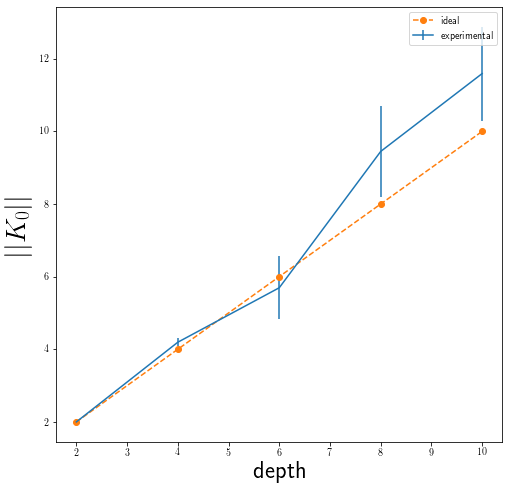
\includegraphics[scale=0.4]{figs/dln-k-vs-d.png}
&
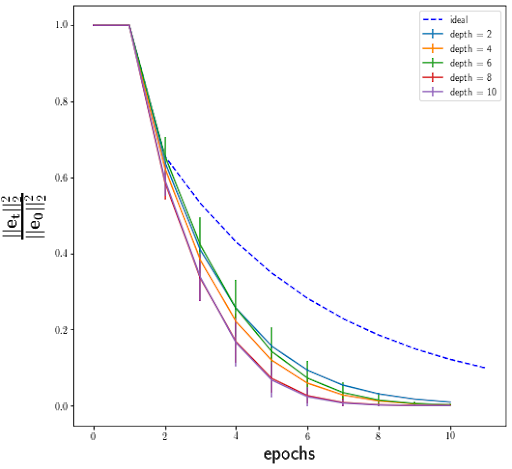
\includegraphics[scale=0.4]{figs/dln-conv.png}
&
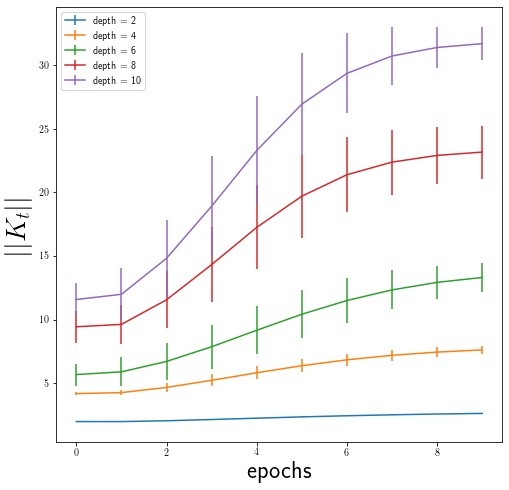
\includegraphics[scale=0.4]{figs/dln-gram.png}
&
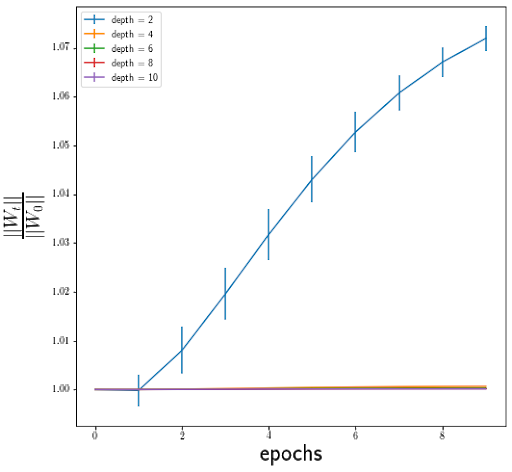
\includegraphics[scale=0.4]{figs/dln-norm.png}
\end{tabular}
}
\caption{In all the plots $d_{in}=1, n=1, w=100,\sigma^2=\frac{1}{w}$ averaged over $5$ runs. The left most plot shows $K_0$ as a function of depth. The second from left plot shows the convergence rate. The third plot from left shows the growth of $K_t$ over the course of training, and the right most plot shows the growth of weights ($L_2$-norm) with respect to time.}
\label{fig:dln}
\end{figure*}

\comment{\section{DGN-FRG}
\textbf{Effect of $p$} is shown in \Cref{fig:peff}. For $w=100$, we observe that for  the e.c.d.f gets better as the value of $p$ reduces till $p=0.3$, after which it starts degrading. This is due to the fact that the variance gets worse with $\frac{1}p$ (since $\sigma=\sqrt{\frac{1}{pw}}$. It can be seen that for $w=50$ the variance is more and hence the e.c.d.f gets better as we reduce $p$ only till $p=0.4$, after which it starts to degrade.

\FloatBarrier
\begin{figure*}[h]
\resizebox{\columnwidth}{!}{
\begin{tabular}{cc}
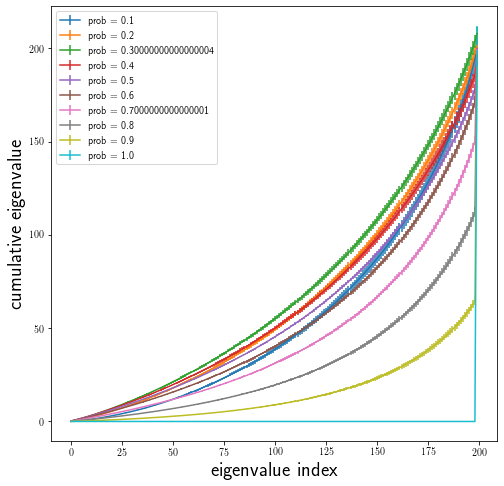
\includegraphics[scale=0.4]{figs/dgn-frg-ecdf-p-w100.png}
&
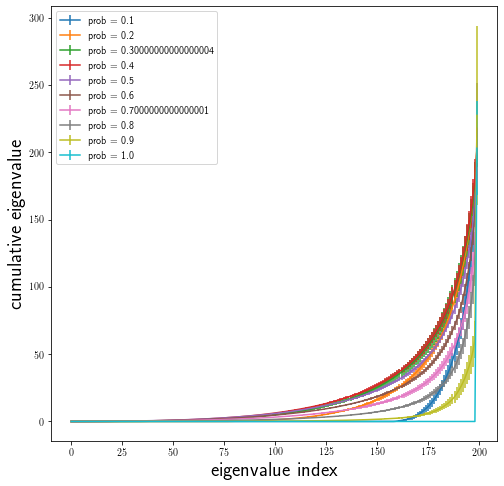
\includegraphics[scale=0.4]{figs/dgn-frg-ecdf-p-w10.png}
\end{tabular}
}
\caption{Shows e.c.d.f for various values of $p$.}
\label{fig:peff}
\end{figure*}}


\textbf{Statement and Proof of Lemma~\ref{lm:invariance}}
\begin{lemma}
At $t=0$, under Assumptions~\ref{assmp:mainone},\ref{assmp:maintwo}, convolutional layers with global average pooling at the end causes translational invariance.
\begin{align*}
&\E{x_s(L,1)x_{s'}(L,1)}\\&=\frac{\sigma^{2(d-1)}}{d^2_{in}}\sum_{k=1}^{\hat{B}} \sum_{p_1,p_2\in b_k}  \Big( x(p_1(0),s) A(x_s,p_1)\\
&\quad\quad \quad\quad \quad\quad x(p_2(0),s') A(x_{s'},p_2) \Big)
\end{align*}
\end{lemma}

\begin{proof}
\begin{align*}
\E{x_s(L,1)x_{s'}(L,1)}&=\E{\phi^\top_{x_s,\G_0} w_0w_0^\top \phi^\top_{x_{s'},\G_0}}\\
&=\phi^\top_{x_s,\G_0}\E{ w_0 w_0^\top} \phi^\top_{x_{s'},\G_0},
\end{align*}
where we use the fact that the gates $\G_0$ are statistically independent of the weights. Now let $M=\E{ w_0 w_0^\top}$, we make the following observations about $M$:

$1.$ $M(p_1,p_2)=0$, if $p_1$ and $p_2$ belong to the different bundles.

$2.$ $M(p_1,p_2)=\frac{\sigma^{2(d-1)}}{d^2_{in}}$, if $p_1$ and $p_2$ belong to the same bundle.

Using the above two observations, we have at  $t=0$:

\begin{align*}
&\E{x_s(L,1)x_{s'}(L,1)}\\&=\phi^\top_{x_s,\G_0} M \phi^\top_{x_{s'},\G_0}\\
&=\sum_{p_1,p_2=1}^{\hat{P}} \Big(x(p_1(0),s) A(x_s,p_1) \\
&\quad\quad \quad\quad \quad\quad x(p_2(0),s') A(x_{s'},p_2) M(p_1,p_2)\Big)\\
&=\frac{\sigma^{2(d-1)}}{d^2_{in}}\sum_{k=1}^{\hat{B}} \sum_{p_1,p_2\in b_k}  \Big( x(p_1(0),s) A(x_s,p_1)\\
&\quad\quad \quad\quad \quad\quad x(p_2(0),s') A(x_{s'},p_2) \Big)
\end{align*}
\end{proof}





\end{document}
